%% 
%% Copyright 2007-2020 Elsevier Ltd
%% 
%% This file is part of the 'Elsarticle Bundle'.
%% ---------------------------------------------
%% 
%% It may be distributed under the conditions of the LaTeX Project Public
%% License, either version 1.2 of this license or (at your option) any    
%% later version.  The latest version of this license is in
%%    http://www.latex-project.org/lppl.txt
%% and version 1.2 or later is part of all distributions of LaTeX
%% version 1999/12/01 or later.
%% 
%% The list of all files belonging to the 'Elsarticle Bundle' is
%% given in the file `manifest.txt'.
%% 
%% Template article for Elsevier's document class `elsarticle'
%% with harvard style bibliographic references

%\documentclass[preprint,12pt]{elsarticle}
\documentclass[11pt,a4paper]{article}

%% Use the option review to obtain double line spacing
%% \documentclass[preprint,review,12pt]{elsarticle}

%% Use the options 1p,twocolumn; 3p; 3p,twocolumn; 5p; or 5p,twocolumn
%% for a journal layout:
%% \documentclass[final,1p,times]{elsarticle}
%% \documentclass[final,1p,times,twocolumn]{elsarticle}
%% \documentclass[final,3p,times]{elsarticle}
%% \documentclass[final,3p,times,twocolumn]{elsarticle}
%% \documentclass[final,5p,times]{elsarticle}
%% \documentclass[final,5p,times,twocolumn]{elsarticle}

%% For including figures, graphicx.sty has been loaded in
%% elsarticle.cls. If you prefer to use the old commands
%% please give \usepackage{epsfig}

%% The amssymb package provides various useful mathematical symbols
\usepackage{amssymb}
%% The amsthm package provides extended theorem environments
%% \usepackage{amsthm}

%% The lineno packages adds line numbers. Start line numbering with
%% \begin{linenumbers}, end it with \end{linenumbers}. Or switch it on
%% for the whole article with \linenumbers.
%% \usepackage{lineno}



\voffset=-1.5cm \hoffset=-1.4cm \textwidth=16cm \textheight=22.0cm
\usepackage[activate={true,nocompatibility},final,tracking=true,kerning=true,spacing=true,factor=1100,stretch=10,shrink=10]{microtype}
\hbadness=99999
\hfuzz=999pt 
\sloppy
\usepackage[utf8]{inputenc}
\usepackage[T1]{fontenc}
\usepackage{babel}

\RequirePackage[sort&compress,numbers]{natbib}
\bibliographystyle{elsarticle-num-names}
%\RequirePackage[sort&compress,numbers]{natbib}

%\bibliographystyle{config/bibstyle}

\renewcommand{\bibfont}{\small}
\usepackage{graphicx,color}
\usepackage{amsmath}
\usepackage[version=4]{mhchem}
\usepackage{siunitx}
\usepackage{longtable,tabularx}
\setlength\LTleft{0pt} 
\usepackage{subcaption}
\usepackage{hyperref}
\usepackage{ragged2e}
\usepackage{arydshln}
\usepackage{optidef} % to write optimization problems
\usepackage[ruled,vlined]{algorithm2e}  % to write algorithms
\usepackage{mathrsfs}   % to write cursive letters
\usepackage{changepage}   % to prevent overfull box
\usepackage{float} 
\usepackage{dsfont}
\usepackage{nccmath}
\usepackage{tabularx}
\usepackage{booktabs}
\usepackage{longtable}
\usepackage{enumitem}
\usepackage{adjustbox}
\usepackage{amsmath}               
\usepackage{amsfonts}               
\usepackage{stanli}
% New command to refer to equations as Eq.(1), Eq.(2), ...
\newcommand{\eqnref}[1]{Eq.~(\ref{#1})}
% New command to refer to figures as Fig.1, Fig.2, ...
\newcommand{\figref}[1]{Fig.~\ref{#1}}
% New command to refer to tables as Tab.1, Tab.2, ...
\newcommand{\tabref}[1]{Tab.~\ref{#1}}
% New command to refer to algorithms as Alg.1, Alg.2, ...
\newcommand{\algref}[1]{Alg.~\ref{#1}}

\newcommand*\samethanks[1][\value{footnote}]{\footnotemark[#1]}

\usepackage{bm}

\usepackage{optidef} % to write optimization problems
\usepackage[ruled,vlined]{algorithm2e}  % to write algorithms
\usepackage{mathrsfs}   % to write cursive letters
\usepackage{changepage}   % to prevent overfull box
\usepackage{float} 
\usepackage{dsfont}
\let\openbox\relax
\usepackage{amsthm}
\usepackage{relsize}

\usepackage{nomencl}
\usepackage{multicol}
\setlength\columnsep{1cm}
\renewcommand{\nompreamble}{\begin{center}\begin{multicols}{2}}
\renewcommand{\nompostamble}{\end{multicols}\end{center}}
\setlength{\nomlabelwidth}{-0.1cm}
\setlength{\nomitemsep}{-0.15\parsep}
\makenomenclature
\providetoggle{nomsort}
\settoggle{nomsort}{true} % true = sort by use, false = sort as usual
\makeatletter
\iftoggle{nomsort}{%
    \let\old@@@nomenclature=\@@@nomenclature        
        \newcounter{@nomcount} \setcounter{@nomcount}{0}%
        \renewcommand\the@nomcount{\two@digits{\value{@nomcount}}}% Ensure 10>01
        \def\@@@nomenclature[#1]#2#3{% Taken from package documentation
          \addtocounter{@nomcount}{1}%
        \def\@tempa{#2}\def\@tempb{#3}%
          \protected@write\@nomenclaturefile{}%
          {\string\nomenclatureentry{\the@nomcount\nom@verb\@tempa @[{\nom@verb\@tempa}]%
          \begingroup\nom@verb\@tempb\protect\nomeqref{\theequation}%
          |nompageref}{\thepage}}%
          \endgroup
          \@esphack}%
      }{}
\makeatother      

\def\abs#1{\left\lvert#1\right\rvert}

\usepackage{xpatch}
\makeatletter
\xpatchcmd\SetKwInOut
  {\hangafter=1\parbox[t]}
  {\hangafter=1\justify\parbox[t]}
  {}{\fail}
\makeatother

\SetKwInOut{Input}{Input}
\DontPrintSemicolon

%to comment some large parts
\usepackage{comment}

 \def\emailname{E-mail}%
\def\email#1{\emailname: #1}
 \def\keywordname{{\bfseries Keywords}}%
  \def\andname{and}%
%remove when submitting:
%\usepackage{showlabels}
\newcounter{countana}


\newcommand{\tstar}[5]{% inner radius, outer radius, tips, rot angle, options
\pgfmathsetmacro{\starangle}{360/#3}
\draw[#5] (#4:#1)
\foreach \x in {1,...,#3}
{ -- (#4+\x*\starangle-\starangle/2:#2) -- (#4+\x*\starangle:#1)
}
-- cycle;
}





\begin{document}
\newtheorem{assumption}{Assumption}
\newtheorem{theorem}{Theorem}
\newtheorem{corollary}{Corollary}
\newtheorem{lemma}{Lemma}
\newtheorem{remark}{Remark}


\date{}

\title{A mixed-categorical correlation kernel for Gaussian process}

\author{
P. Saves\thanks{ONERA/DTIS \& ISAE-SUPAERO, Universit\'e de Toulouse, France. \email{{\tt paul.saves@isae-supaero.fr}}
}
\and
Y. Diouane\thanks{MAGI, Polytechnique Montr\'eal, Canada. \email{{\tt youssef.diouane@polymtl.ca}}
}
\and
N. Bartoli\thanks{ONERA/DTIS, Universit\'e de Toulouse, France. \email{{\tt nathalie.bartoli@onera.fr}}
}
\and
T. Lefebvre\thanks{ONERA/DTIS,  Universit\'e de Toulouse, France. \email{{\tt thierry.lefebvre@onera.fr}}
}
\and
J. Morlier\thanks{ICA, Universit\'e de Toulouse, ISAE-SUPAERO, MINES ALBI, UPS, INSA, CNRS, Toulouse, France. \email{{\tt joseph.morlier@isae-supaero.fr}}
}
}

\maketitle
\footnotesep=0.4cm


\begin{abstract}
Recently, there has been a growing interest for mixed-categorical meta-models based on Gaussian process (GP) surrogates. In this setting, several existing approaches use different strategies either by using continuous kernels (\textit{e.g.}, continuous relaxation and Gower distance based GP) or by using a direct estimation of the correlation matrix. 
In this paper, we present a kernel-based approach that extends continuous exponential kernels to handle mixed-categorical variables. The proposed kernel leads to a new GP surrogate that generalizes both the continuous relaxation and the Gower distance based GP models. 
We demonstrate, on both analytical and engineering problems, that our proposed GP model gives a higher likelihood and a smaller residual error than the other kernel-based state-of-the-art models. Our method is available in the open-source software SMT. 
\end{abstract}

%%Graphical abstract

%\begin{graphicalabstract}
%\includegraphics{grabs}
%\end{graphicalabstract}

%%Research highlights
%\begin{highlights}
%\item Research highlight 1
%\item Research highlight 2
%\end{highlights}

%\begin{keyword}
%% keywords here, in the form: keyword \sep keyword

%% PACS codes here, in the form: \PACS code \sep code

%% MSC codes here, in the form: \MSC code \sep code
%% or \MSC[2008] code \sep code (2000 is the default)

%\end{keyword}




% %\section{Nomenclature}
%  \nomenclature{$n$   : }{ number of continuous variables }  
% \nomenclature{$m$   : }{ number of integer variables }
% \nomenclature{$l$   : }{ number of categorical variables }
% \nomenclature{$\Omega \subset  \mathbb{R}^n$   : }{ continuous space }
% \nomenclature{$S \subset \mathbb{Z}^m$   : }{ integer space }
% \nomenclature{$\mathbb{F}^l$   : }{ categorical space }

% \nomenclature{$L_i$   : }{ number of levels for the  $i^{th}$ categorical variable, $i \in \{1,\ldots, l\} $ }

 
% \nomenclature{$\theta^{cont}$   : }{ vector of hyperparameters for the continuous part of the Gaussian process } 
% %\nomenclature{$k^{cont}$   : }{ continuous correlation kernel }
% %\nomenclature{$\theta^{cont}_j$   : }{ hyperparameter  for the  $j^{th}$ continuous variable, $ j \in \{1,\ldots, n\} $ } 
% \nomenclature{$R^{cont}$   : }{ correlation matrix for continuous inputs } 

% \nomenclature{$\theta^{int}$   : }{ vector of hyperparameters for integer inputs} 
% %\nomenclature{$k^{int}$   : }{ integer correlation kernel }
% %\nomenclature{$\theta^{int}_j$   : }{ hyperparameter  for the  $j^{th}$ integer variable, $ j \in \{1,\ldots, m\} $ } 
% \nomenclature{$R^{int}$   : }{ correlation matrix for integer inputs } 

% \nomenclature{$\theta^{cat}$   : }{ hyperparameters for categorical inputs} 
% %\nomenclature{$R_i $   : }{ correlation matrix for the  $i^{th}$ categorical variable }
% %\nomenclature{$\Theta_i $   : }{ matrix of hyperparameters  for the  $i^{th}$ categorical variable }
% \nomenclature{$R^{cat}$   : }{ correlation matrix for categorical inputs } 

% \nomenclature{$\Theta=\{\theta^{cont}, \theta^{int}, \theta^{cat} \}$   : }{ hyperparameters for the Gaussian process model } 
% \nomenclature{$R=R^{cont}R^{int}R^{cat}$   : }{ correlation matrix for mixed-categorical inputs }  

% %\nomenclature{$d$   : }{ number of PLS-reduced continuous dimensions } 
% %\nomenclature{$\hat{\theta}_t^{cont}$   : }{ hyperparameter  for the $t^{th}$ PLS-reduced continuous dimension, $ t \in \{1,\ldots, d\} $ } 
% %\nomenclature{$\lambda_j^{cont}$   : }{ hyperparameter approximation  for the  $j^{th}$ continuous variable } 
% %\nomenclature{$g_{*j}^{(t)}$   : }{ value of the PLS rotation vector for principal component $t$ } 

% %\nomenclature{$\ell_i$   : }{ number of PLS-reduced  levels for the  $i^{th}$ categorical variable } 

% %\nomenclature{$\hat{\Theta}_i$   : }{ matrix of  PLS-reduced hyperparameters for the $i^{th}$ categorical variable } 
% %\nomenclature{$\Lambda_i$   : }{ hyperparameters matrix approximation for the  $i^{th}$ categorical variable } 
% \printnomenclature

% % {\renewcommand\arraystretch{1.0}
% % \noindent\begin{longtable*}{@{}l @{\quad=\quad} l@{}}
% % $n$ & number of continuous variables \\
% % $m$ & number of integer variables \\
% % $l$ & number of categorical variables \\
% % $\Omega \subset  \mathbb{R}^n$ & continuous space\\
% % $S \subset \mathbb{Z}^m$  & integer space \\
% % $\mathbb{F}^l$ & categorical space \\

% % $L_i, i \in \{1,\ldots, l\} $ & number of levels for the  $i^{th}$ categorical variable \quad \quad \quad \quad \quad \quad \quad \quad \quad \quad \quad \quad \\

 
% % $\theta^{cont}$  &  vector of hyperparameters for the continuous part of the Gaussian process   \\ 
% % $k$ & correlation kernel \\
% % $\theta^{cont}_j, j \in \{1,\ldots, n+m\} $  &  hyperparameter  for the  $j^{th}$ continuous or integer variable  \\ 
% % $R^{cont}$ & correlation matrix for continuous and integer inputs \\ 


% % $\theta^{cat}$  &  hyperparameters for the categorical part of the Gaussian process model  \\ 
% % $K_i $ &   categorical kernel for the  $i^{th}$ categorical variable  \\
% % $\Theta_i $  &   matrix of hyperparameters  for the  $i^{th}$ categorical variable  \\
% % $R^{cat}$ & correlation matrix for categorical inputs \\ 

% % $\Theta=[\theta^{cat}, \theta^{cont}]$&  hyperparameters for the Gaussian process model  \\ 
% % $R=R^{cont}R^{cat}$ & correlation matrix for mixed integer inputs \\ 


% % \end{longtable*}}

% %%%%%%%

%\tableofcontents
%\newpage

%%%%%%

%%----------------------------------------------------------------------
%%% INTRODUCTION
%----------------------------------------------------------------------
% !TEX root = ../Main.tex


\Acp{BPM} have a long and rich history in optimization, going back at least to the introduction of \acl{MD} by Nemirovski \& Yudin \citep{NY83}.
In plain terms, \acp{BPM} are first-order (constrained) optimization algorithms that forego Euclidean projections in favor of a more sophisticated ``prox-mapping'' that minimizes a certain distance-like functional known as the Bregman divergence \citep{NY83,CT93,Bre67,Kiw97}.
When this Bregman divergence is the Euclidean distance squared, one recovers the standard projection-based methods;
other than that, depending on the problem's feasible region, different Bregman setups lead to a diverse collection of algorithms,
from exponentiated gradient descent on the simplex \citep{NY83,BecTeb03,ACBFS02},
to matrix multiplicative weights on the positive-semidefinite cone \cite{TRW05,KSST12},
variants of Karmarkar's affine scaling algorithm for linear programs \cite{VMF86},
etc.

One of the most appealing features of \acp{BPM} is that they achieve almost dimension-free convergence rates in problems with a convex structure and a favorable geometry \textendash\ such as the $L^{1}$ ball, the spectraplex, second-order cones, etc. \cite{Bub15,Nes09,BecTeb03}.
This is owed to a delicate interplay between the algorithms' non-Euclidean update scheme and the global geometry of the problem's domain.
However, these (almost) dimension-free guarantees also come with some strings attached:
they do not concern the sequence of iterates generated by the method, but only its time average
\revise{(or, through the same, ``regret-based'' analysis, the method's ``best iterate'')};
in this way, the best guarantee that can be achieved after $\run$ iterations is $\bigoh(1/\run)$.

In terms of oracle complexity, this is sufficient for problems that are not strongly convex\,/\,strongly monotone, but if one targets finer, geometric convergence rates,
\revise{the inherent averaging involved in regret-based guarantees is hard to compensate.}
And, on the other extreme, if the problem is not convex\,/\,monotone to begin with, iterate averaging does not provide any quantifiable benefits whatsoever, so it becomes crucial to study the actual trajectory of the method.


%----------------------------------------------------------------------
%%% CONTRIBS
%----------------------------------------------------------------------
\para{Our contributions}

Our paper seeks to quantify the last-iterate convergence rate of \aclp{BPM} as a function of the Bregman divergence defining the method and the local geometry that it induces.
To treat this question in as general a manner as possible, we focus on \ac{VI} problems of the form
\begin{equation}
\label{eq:VI}
\tag{VI}
\text{Find $\sol\in\points$ such that}
	\;\;
	\braket{\vecfield(\sol)}{\point - \sol}
	\geq 0
	\;\;
	\text{for all $\point\in\points$},
\end{equation}
where $\points$ is a closed convex subset of a finite-dimensional normed space $\pspace$, and $\vecfield \from \points \to \dspace$ is a (possibly non-monotone) single-valued operator on $\points$ with values in $\dspace$, the dual of $\pspace$.
This problem is a staple of many areas of mathematical programming, game theory and data science, as it provides a template for ``optimization beyond minimization'' \textendash\ \ie for problems where finding an optimal solution does not necessarily involve minimizing a loss function.
In particular, in addition to standard minimization problems \textendash\ which are recovered when $\vecfield = \nabla\obj$ for some smooth function $\obj$ \textendash\ the general formulation \eqref{eq:VI} includes saddle-point problems, games, complementarity problems, etc.;
for an introduction, see \cite{FP03} and references therein.

In this broad context, we examine the rate of convergence of a wide class of \aclp{BPM} to local solutions of \eqref{eq:VI} that satisfy a \acl{SOS} condition.
Specifically, the class of algorithms we consider includes as special cases
\begin{enumerate*}
[(\itshape i\hspace*{1pt}\upshape)]
\item
the original \acf{MD} algorithm of \cite{NY83};
\item
the \acf{MP} method of Nemirovski \cite{Nem04} \textendash\ which has the same update structure as the Bregman-based algorithm of \cite{AT05} and contains as a special case the \acf{EG} algorithm of \cite{Kor76};
\item
the so-called \acf{OMD} method of \cite{RS13-NIPS} \textendash\ itself a Bregman analogue of the modified Arrow-Hurwicz algorithm of \cite{Pop80};
\end{enumerate*}
etc.

Our first finding is a crisp characterization of last-iterate convergence rate of \acp{BPM} in terms of the local geometry induced by the underlying Bregman function near a given solution of \eqref{eq:VI}.
We make this dependence precise via the notion of the \emph{Legendre exponent}, a regularity measure for Bregman methods due to \cite{AIMM21}, which can roughly be described as the logarithmic ratio of the volume of a Euclidean ball to that of a Bregman ball of the same radius.
For example, Euclidean methods have a Legendre exponent of $\legexp = 0$ and they converge at a linear rate;
entropic methods have a Legendre exponent of $\legexp = 1/2$ at boundary points, and they converge at a rate of $\bigoh(\run^{-1})$;
more generally,
as we show in \cref{thm:general}, methods with a Legendre exponent $\legexp>0$ converge at a rate of $\bigoh(\run^{1-1/\legexp})$.
\PM{We need to fix this: the $1-1/\legexp$ exponent is not consistent with the $\bigoh(1/\run)$ expression.}
\WA{I don't see the issues, yes this expression is not well-defined for $\legexp = 0$ but this is normal, the two situations differ radically.}
The Euclidean regime ($\legexp = 0$) is perfectly aligned with existing results for the geometric last-iterate convergence rate of the \ac{EG} algorithm and its variants \citep{GBVV+19,Mal15,HIMM19,MOP20}.
By contrast, the Legendre regime ($\legexp > 0$) indicates a significant drop in the algorithm's last-iterate convergence speed, even though ergodic convergence rates \cite{Nes04} and results for bilinear games \cite{WLZL21} might suggest otherwise.

Subsequently, motivated by applications to game theory and linear programming, we take a closer look at the convergence rate of \acp{BPM} across the constraints that are active at a solution $\sol$ of \eqref{eq:VI} depending on the position of $\vecfield(\sol)$ relative to said constraints. 
This analysis reveals that Bregman proximal methods have a particularly fine structure:
along \emph{sharp directions} (\ie constraints along which $\vecfield(\sol)$ is strictly inward-pointing), \acp{BPM} converge
\begin{enumerate*}
[(\itshape i\hspace*{1pt}\upshape)]
\item
at a rate of $\bigoh(1/\run^{1/(2\legexp-1)})$ if $1/2 < \legexp < 1$;
\item
at a \emph{geometric rate} if $0 < \legexp \leq 1/2$ (\eg for entropic methods);
and
\item
in a \emph{finite} number of iterations if $\legexp=0$
\end{enumerate*}
(\cf \cref{thm:sharp}).
Thus, even though the estimates of \cref{thm:general} are, in general tight, the actual convergence rate of a Bregman method along different coordinates\,/\,constraints could be starkly different \textendash\ and, in fact, dramatically faster if the solution under study is itself sharp.

The closest antecedent of our work is the conference paper \cite{AIMM21} where the Legendre exponent was introduced to analyze the convergence of \ac{OMD} in \emph{stochastic} \ac{VI} problems (without considering sharp directions and/or faster identification rates).
The stochastic and deterministic settings are obviously very different, both in the challenges involved as well as the rates obtained, so there is no overlap in our analysis and results.
Other than that, we are not aware of any comparable results in the literature concerning the radically different convergence landscape of \acp{BPM} along active and inactive constraints.
\section{Introduction}
\renewcommand*\footnoterule{}

\label{sec:intro}

%\quad \quad  New aircraft configurations with a lower footprint on the environment (also known as Eco-aircraft design) have seen a resurgence of interest \cite{Eco-material,SEGO-UTB-Bombardier,AGILE}. In this context, one targets to minimize the footprint on the environment of the aircraft using a \textit{Multidisciplinary Design Analysis} (MDA)~\cite{Lambe2011,Lambe2012,Lambe2013}. This is an example of an expensive-to-evaluate without derivative problem that could be encountered on industry. Therefore, it could be useful to use a surrogate model that simplifies by a lot an expensive model and gives a good approximation from a small data set of known configurations. 
%Nevertheless, in this context, the process generally involves mixed continuous-categorical design variables. For instance, the size of aircraft structural parts can be described using continuous variables; in case of thin-sheet stiffened sizing, they represent panel thicknesses and stiffening cross-sectional areas. The set of discrete variables can encompass design variables such as the number of panels, the list of cross sectional areas or the material choices. \\
Expensive-to-evaluate blackbox simulations play a key role for many engineering and industrial applications. In this context, surrogate models have shown great interest for a wide range of applications, \textit{e.g.}, aircraft design~\cite{SciTech_cat}, deep neural networks~\cite{snoek2015scalable}, coastal flooding prediction~\cite{lopez}, agriculture forecasting~\cite{MLP} or seismic imaging~\cite{YDiouane_SGratton_XVasseur_LNVicente_HCalandra_2016}.
These blackbox simulations are generally complex and may involve mixed-categorical input variables. Typically, an aircraft design tool has to take into account variables such as the number of panels, the list of cross sectional areas or the material choices.
%Typically, a deep learning model has to take into account categorical variables (in addition to continuous ones) such as the number of hidden layers or the list of available activation functions (e.g., Linear, Sigmoid, Tanh, ReLU). 

In this work, we target to learn an inexpensive surrogate model $ \hat{f}$ from a mixed-categorical blackbox function given by
\begin{equation}
f :  \Omega \times S \times \mathbb{F}^l \to \mathbb{R}.
  \label{eq:opt_prob}
\end{equation}
This function $f$ is typically an expensive-to-evaluate simulation with no exploitable derivative information.
 $\Omega \subset \mathbb{R}^n$ represents the bounded continuous design set for the $n$ continuous variables.  $S \subset \mathbb{Z}^m$ represents the bounded integer set where $L_1, \ldots, L_m$ are the numbers of levels of the $m$ quantitative integer variables on which we can define an order relation and $ \mathbb{F}^l = \{1, \ldots, L_1\} \times \{1, \ldots, L_2\} \times  \ldots \times \{1, \ldots, L_l\}$ is the design space for the $l$ categorical qualitative variables with their respective  $L_1, \ldots, L_l$ levels.

For that purpose, \textit{Gaussian process} (GP)~\cite{williams2006gaussian}, also called Kriging model~\cite{krige1951statistical}, is known to be a good modeling strategy to learn a response surface model from a given dataset. Namely,
we will consider that our unknown blackbox function $f$ follows a Gaussian process of mean $\mu^{f}$ and of standard deviation $\sigma^f$, $\textit{i.e.}$,
\begin{equation}
f \sim \hat{f}=\mbox{GP}\left(\mu^{f}, [\sigma^f]^2\right). \label{eq:GP:f}\end{equation}
For a general problem involving categorical or integer variables, several modeling strategies to build a mixed-categorical GP have been proposed~\cite{Pelamatti, Zhou, Deng, Roustant,GMHL,Gower,cuesta2021comparison,SciTech_cat}. Compared to a continuous GP, the major changes are in the estimation of the correlation matrix, the latter being essential to build estimates of $\mu^{f}$ and $\sigma^f$. Similarly to the process of constructing a GP with continuous inputs, relaxation techniques~\cite{GMHL,SciTech_cat}, continuous latent variables~\cite{cuesta2021comparison} and Gower distance based models~\cite{Gower} use a kernel-based approach to estimate the correlation matrix.
Other recent approaches try to estimate the correlation matrix independently of a kernel choice by modeling  directly the possible correlation entries of the correlation matrix~\cite{Pelamatti, Zhou, Deng, Roustant}.

Using GP surrogates is not the only possible approach whatsoever. Random forests are often used instead of GP as they also can model both mean and variance~\cite{SMAC} and tree-structured Parzen estimators have been shown to be well-adapted for such problems~\cite{TPE}. Other surrogate models for blackbox include ReLU functions~\cite{Relu-surr}, piecewise linear neural network~\cite{nn-surr} or categorical regression splines~\cite{splines}. Models other than GP could also be based on a mixed integer kernel as for support vector regression~\cite{herrera} or on a mixed integer distance as for radial basis functions~\cite{RBF_geo}. Another classical modeling strategy is to consider a different continuous model for every possible categorical choice and to build another model peculiar to the categorical variables besides the continuous models. This categorical model can be, for instance, a probability law~\cite{CAT-EGO}, a multi-arm bandit~\cite{Bandit-BO} or an integer model~\cite{AMIEGO}. Also, in case of prior information, latent variables approaches~\cite{cuesta2021comparison} and user-defined neighbourhood~\cite{Mixed_Abramson} based models are of great interest, especially for engineering problems.

In this paper, we target to extend the classical paradigm for continuous inputs (where a kernel is used to build the GP) to cover the mixed-categorical case. Namely, we will present a kernel-based approach that will lead to a unified model for existing approximation strategies~\cite{Pelamatti, GMHL,Gower}. This work generalizes existing methods that were already proven to be efficient over deep learning models~\cite{GMHL} and analytical test cases~\cite{Gower}. 
A similar kernel for the estimation of the correlation matrix could be applied to continuous, integer and categorical inputs. The good potential of the proposed approach is shown and analyzed over analytical and industrial test cases.

The GP models and the Bayesian Optimization (BO) that could be performed with them are implemented in the Surrogate Modeling Toolbox (SMT) v1.4\footnote{\url{https://smt.readthedocs.io/en/latest/}}. The latter modeling toolbox is developed by ONERA, ISAE-Supaero, ICA (CNRS), NASA Glenn and the University of Michigan~\cite{SMT2019}. Our modeling software is free and open-source and has been used regularly in the aircraft industry, for example with a deep learning model~\cite{DL1, DL2, DL3, DL4} or with a deep gaussian process~\cite{DGP1,DGP2}. 
%These surrogate models are generally used for the Bayesian Optimization (BO) of a complex system, typically for hyperparameters optimization in the context of deep learning, as for AlphaGo~\cite{chen2018bayesian}. 

The reminder of this paper is as follows.
In Section~\ref{sec:GP}, a detailed review of the GP model for continuous and for categorical inputs is given.
The extended kernel-based approach for constructing the correlation matrix is presented in Section~\ref{sec:model_uni}.
Section~\ref{sec:Results} presents academical tests as well as the obtained results.
Conclusions and perspectives are finally drawn in Section~\ref{sec:conclu}.

%\input{GP categorical}
\section{GP for mixed-categorical inputs}
\renewcommand{\footnoterule}{ \hrule width5cm \vspace*{0.1cm} }    
\label{sec:GP}

In this section, we will present the mathematical background associated with GP for mixed-categorical variables. This part also introduces the notations that will be used throughout the paper. In this section, we are considering the general case involving mixed integer variables. Namely, we assume that $f:\mathbb{R}^n \times  \mathbb{Z}^m \times \mathbb{F}^l \mapsto \mathbb{R}$ and our goal is to build a GP surrogate model for $f$. 

%\subsection{Background on Gaussian process interpolation}
Given a set of data points, called a Design of Experiments (DoE)~\cite{forrester}, Bayesian inference learns the GP model that explains the best this data set. A GP model consists of a mean response hypersurface $\mu^{f}$, as well as an estimation of its variance $[\sigma^f]^2$. In the following, $n_t$ denotes the size of the given DoE data set $(W, \textbf{y}^f)$ such that $W=\{w^1,w^2,\ldots,w^{n_t}\} \in (\mathbb{R}^n \times  \mathbb{Z}^m \times \mathbb{F}^l)^{n_t}$ and $\textbf{y}^f=[f(w^1),f(w^2),\ldots,f(w^{n_t})]^{\top}$. 
For an arbitrary $w= (x,z,c) \in \mathbb{R}^n \times  \mathbb{Z}^m \times \mathbb{F}^l$, not necessary in the DoE, the GP model prediction at $w$ writes as $\hat f(w) = \mu ({w})+\epsilon(w) \in \mathbb{R} $, with $\epsilon$ being the error between $f$ and the model approximation $\mu$~\cite{GP14}. The considered error terms are random variables of variance $\sigma^2$.  Using the DoE, the expression of  $\mu^{f}$ and the estimation of its variance $[\sigma^f]^2$ are given as follows:

\begin{equation} \label{eq:mean:GP}
\mu^f(w)= \hat{\mu}^f+r(w)^\top  [R(\Theta)]^{-1}(\textbf{y}^f-\mathds{1} \hat{\mu}^f), 
\end{equation}
and
\begin{equation}
\label{eq:std:GP}
[\sigma^f(w)]^2=[\hat{\sigma}^f]^2\left[1-r(w)^\top  [R(\Theta)]^{-1}r(w)+ \frac{ \left(1-\mathds{1}^\top  [R(\Theta)]^{-1}r(w) \right)^2}{\mathds{1}^\top  [R(\Theta)]^{-1}\mathds{1}}\right], \end{equation}
where $\hat{\mu}^f$ and $\hat{\sigma}^f$, respectively, are the maximum likelihood estimator (MLE)~\cite{MLE} of $\mu$ and $\sigma$. $\mathds{1}$ denotes the vector of $n_t$ ones. $R$ is the $ n_t \times n_t $ correlation matrix between the input points and $r(w)$ is the correlation vector between the input points and a given $w$.
The correlation matrix $R$ is defined, for a given couple  $(r,s) \in (\{1,\ldots,n_t\})^2$, by \begin{equation}
\label{eq:R}
 [R(\Theta)]_{r,s}=k\left(w^r,w^s,\Theta\right) \in \mathbb{R},\end{equation}
and the vector $r(w)\in \mathbb{R}^{n_t}$ is defined as $ r(w) =[k(w,w^1), \ldots , k(w,w^{n_t})]^{\top}$,
where $k$ is a given correlation kernel that relies on a set of hyperparameters $\Theta$~\cite{Roustant}. 
The mixed-categorical  correlation kernel is given as the product of three kernels:
\begin{equation}
k(w^r,w^s,\Theta) =  k^{cont}\left(x^r,x^s,\theta^{cont}\right) k^{int}\left(z^r,z^s,\theta^{int}\right)
k^{cat}\left(c^r,c^s,\theta^{cat}\right),
\label{eq:decomp_mix}
\end{equation}
%with $.$ being in this case the product, even if one could choose to use a sum or a ANOVA~\cite{roustant_hal}. 
where $k^{cont}$  and $\theta^{cont}$ are the continuous kernel and its associated hyperparameters, $k^{int}$  and $\theta^{int}$ are the integer kernel and its hyperparameters, and last $k^{cat}$  and $\theta^{cat}$ are the ones related with the categorical inputs. In this case, one has $\Theta=\{ \theta^{cont},\theta^{int},\theta^{cat}\}$. 
Henceforth, the general correlation matrix $R$ will rely only on the set of the hyperparameters $\Theta$:
\begin{equation}
    \label{eq:corel:mat}
    [R(\Theta)]_{r,s} = [R^{cont}(\theta^{cont})]_{r,s}  [R^{int}(\theta^{int})]_{r,s}
    [R^{cat}(\theta^{cat})]_{r,s},
\end{equation}
where $[R^{cont}(\theta^{cont})]_{r,s} =k^{cont}(x^r,x^s,\theta^{cont}) $, $[R^{int}(\theta^{int})]_{r,s} =k^{int}(z^r,z^s,\theta^{int}) $ and  $[R^{cat}(\theta^{cat})]_{r,s}=k^{cat}(c^r,c^s,\theta^{cat})$. 
The set of hyperparameters $\Theta$ could be estimated using the DoE data set $({W},\textbf{y}^f)$ through the MLE approach on the following way
\begin{equation}
\Theta^*= \arg\max_{\Theta} \mathcal{L}(\Theta):=\left( - \frac{1}{2} {\textbf{y}^f}^\top [R(\Theta)]^{-1} {\textbf{y}^f}   - \frac{1}{2} \log 	\abs{  [R(\Theta)]} - \frac{n_t}{2} \log 2 \pi    \right),
\label{eq:likelihood}
\end{equation}
where $R(\Theta)$ is computed using~\eqnref{eq:corel:mat}. 
To construct the correlation matrix, several choices for the correlation kernel are possible. Usual families of kernels include exponential kernels or Matern kernels~\cite{Lee2011}. 
In the rest of this section, we will focus mainly on the exponential kernels and describe in details the construction of the continuous $R^{cont}(\theta^{cont})$, the integer $R^{int}(\theta^{int})$ and the categorical $R^{cat}(\theta^{cat})$ correlation matrices. 

\subsection{Correlation matrices for continuous and integer inputs}
\label{sec:GP_cont}


%To begin with, we consider the case in which we assume all the design variables are continuous in problem \eqref{eq:opt_prob} such that the design space is restricted to $\Omega \subset \mathbb{R}^n$. 

%In these formulae, $\hat{f}$ and $[s^f]^2$ both depend on $R$ and $r$ which are characterized by the correlation kernel $k(.,.,\theta^{cont})$.

The construction of the correlation matrix $R^{cont}(\theta^{cont})$ for continuous inputs, based on an exponential kernel, can be described as follows. 
For a couple of continuous inputs $x^r\in \mathbb{R}^n$ and $x^s\in \mathbb{R}^n$, one sets 
\begin{equation}
[R^{cont}(\theta^{cont})]_{r,s}= {\displaystyle \prod_{j=1}^{n}{  \exp \left(-   \theta^{cont}_j  \abs{x^r_j - x^s_j}^p \right) }}. 
\label{eq:E_cont}
\end{equation}
Different values for $p$ can be used. Typically, when $p=1$, one gets the absolute exponential kernel (Ornstein-Uhlenbeck process~\cite{Lee2011}) and, when $p=2$, the squared exponential kernel (or Gaussian kernel~\cite{williams2006gaussian}) is obtained. Clearly, in the continuous case, constructing $R^{cont}(\theta^{cont})$ would require the estimation of $n$ non-negative hyperparameters, $\textit{i.e.}$, $\theta^{cont} \in \mathbb{R}^n_+$.

Thanks to a continuous relaxation technique that transforms integer inputs into continuous ones, the integer inputs can be naturally handled with continuous kernels. On this base, in what comes next, there will be no distinction between continuous and integer inputs; the two of them will be handled in the same way. In fact, for integer variables, the distance defined in the continuous case is still valid. Thus, for an integer couple $z^r\in \mathbb{Z}^m$ and $z^s\in \mathbb{Z}^m$, a natural extension of the exponential kernel that handles integer variables can be given as follows:
\begin{equation}
[R^{int}(\theta^{int})]_{r,s} = {\displaystyle \prod_{{j}=1}^{m}{  \exp \left(-   \theta^{int}_{j}  \abs{z^r_{j} - z^s_{j}}^p \right) }}.
\end{equation}
In a similar fashion, constructing $R^{int}(\theta^{int})$ would require the estimation of $m$ non-negative hyperparameters, $\textit{i.e.}$, $\theta^{int} \in \mathbb{R}^m_+$.

%In the next part, for the general mixed-categorical case, we will consider different models to build the categorical kernel.

\subsection{Correlation matrices for categorical inputs}
\label{subsec:mi_kriging}

For categorical inputs, different choices can be made to build the correlation matrix $R^{cat}(\theta^{cat})$. Some choices are sophisticated and can therefore lead to better GP models, but are known to be computationally expensive (particularly as the number of categorical inputs increases)~\cite{Roustant,Pelamatti}. On the contrary, simple extensions of the well-known continuous kernels based on the Gower distance~\cite{Gower} or on the continuous relaxation techniques~\cite{one-hot} would be less expensive.
In the rest of this section, we will describe three known techniques to build correlation matrices for categorical inputs that are based on kernels. 

\subsubsection{Gower distance based kernel}

The Gower distance based kernel dedicates one hyperparameter per categorical input variable~\cite{Gower,RaulAIAA}. This method uses the notion of Hamming distance between categorical inputs to naturally extend continuous correlation kernel functions. Namely, for two given inputs $c^r \in \mathbb{F}^l$ and $c^s \in \mathbb{F}^l$, the Hamming distance, or score, $s$ between the $i^{th}$ component of $c^r$ and $c^s$ is defined as: $s(c_i^r, c_i^s)=1$ if $c_i^r = c_i^s$, otherwise $s(c_i^r, c_i^s)=0$. Thanks to the Hamming distance, one can straightforwardly uses a continuous kernel  to define $R^{cat}(\theta^{cat})$. For instance, in the case of an exponential kernel, the Gower distance based correlation matrix will be given by 
$$
[R^{cat}(\theta^{cat})]_{r,s} =k^{cat}(c^r,c^s,\theta^{cat}) = {\displaystyle \prod_{i=1}^{l}{   \exp \left(- \theta_i^{cat} s(c_i^r,c_i^s)^p  \right) }}.  
$$
Similarly to the continuous and integer correlation matrices, the construction of the categorical correlation matrix based on the Gower distance kernel requires the estimation of $l$ hyperparameters ($\theta^{cat} \in \mathbb{R}^l_+$). Note that, as the Hamming distance can only takes the values $0$ and $1$, all the exponential kernels lead to the same result independently of the value of $p$.



%As in the continuous case, for a given variable, the corresponding hyperparameter is multiplied by the distance between two inputs points. 
%The integer variables are therefore treated as the continuous ones.
%For two given inputs $c^r$ and $c^s$, the Hamming distance, or score, between $c^r$ and $c^s$ is defined as: 
%\begin{equation*}
% \begin{cases}
%&s(c_i^r, c_i^s)=1, \text{ if } c_i^r = c_i^s \\
%&s(c_i^r, c_i^s)=0,\text{ if }   c_i^r \neq c_i^s \\
%\end{cases}
%\end{equation*}

%$$\Delta_{gow}(w^r,w^s) =   {\displaystyle \sum_{i=1}^{l}{ s(c_i^r, c_i^s) }}  +  {\displaystyle \sum_{j=1}^{n}{ |x_j^r-x_j^s| }}+  {\displaystyle \sum_{{j'}=1}^{m}{ |z_{j'}^r-x_{j'}^s| }}$$
%Where $s$ is the score distance, also called Hamming distance, defined as:


%Hence, the mixed categorical kernel writes as 
%$$
%k(w^r,w^s,\theta) = {\displaystyle \prod_{i=1}^{l}{   \exp \left(- \theta_i^{cat} s(c_i^r,c_i^s)^p  \right) }} {\displaystyle \prod_{j=1}^{n}{   \exp \left(- \theta_j^{cont} |x_j^r - x_j^s |^p  \right) }} {\displaystyle \prod_{{j'}=1}^{n}{   \exp \left(- \theta_{j'}^{cont} |z_{j'}^r - z_{j'}^s |^p  \right) }} 
%$$

%Hence, the categorical correlation matrix writes as 
%$$
%[R^{cat}(\theta^{cat})]_{r,s} =k^{cat}(c^r,c^s,\theta^{cat}) = {\displaystyle \prod_{i=1}^{l}{   \exp \left(- \Theta_i^{cat} s(c_i^r,c_i^s)^p  \right) }}  
%$$
%This kernel relies on $l$ hyperparameters. For this kernel, the value of $p$ is irrelevant as $1^p=1$ and $0^p=0$.

%\input{Unified model}

\subsubsection{Continuous relaxation based kernel}

To handle categorical variables through continuous relaxation, the design space $ \mathbb{F}^l $ is relaxed to a continuous space $ \Omega^l$  constructed in the following way. 
%For all $ i \in \{1, \ldots,l\}$, recall that $L_i$ represents the number of levels associated with $c_i$, that is $i^{th}$ component of the categorical variable $c$, and, at the beginning we set $ \Omega^l$ to be empty. Then, for each $i  \in \{1, \ldots,l\}$, a relaxed one-hot encoding is used~\cite{one-hot} for $c_i$.
%The mapping to a $L_i$-dimensional Hilbert space defined in such a way that the only non-zero coordinate of the image is $1$ in a dimension associated to the mapped level is the so-called one-hot encoding.
For a given $i\in \{1,\ldots,l\}$, let $c_i$ be the $i^{th}$ categorical variable with $L_i$ levels, and, for a given input point $c^r$, let $\ell_r^i$ be the index of the level taken by $c^r$ on the variable $i$.
Denote $e_{c^r_i}$ the one-hot encoding~\cite{one-hot} of $c^r_i$ that takes value $0$ everywhere but on the dimension $\ell_r^i$:  $e_{c^r_i} \in \mathbb{R}^{L_i} $ such that $\left( e_{c^r_i} \right)_{\ell^i_r}=1$ and $\left( e_{c^r_i} \right)_k=0$ for $k \neq \ell^i_r$. 
For example, if the $i^{th}$ component is the color with $L_i=3$ levels being $ \{ \mbox{red}, \mbox{blue}, \mbox{green} \}$ and if the $r^{th}$ variable takes value $\mbox{blue}$ ($c_i^r = \mbox{blue}$), then the corresponding index is $\ell_r^i =2$ and the corresponding one-hot encoding is $e_{c^r_i} = (0,1,0)$.
The continuous relaxation idea is as follows. At the beginning we set $ \Omega^l$ to be empty, then, for each $i  \in \{1, \ldots,l\}$, a relaxed one-hot encoding is used for $c_i$. The latter increases the dimension of the relaxed continuous space $ \Omega^l$ by $L_i$ and, at the end of the relaxation, we get the final continuous design space $\Omega^l\subseteq \{0,1\}^{n^l}$, where $n^l=\sum_{i=1}^l L_i >l$. 
%Due to the one-hot encoding, the final relaxed design space is of the form
%$
%\Omega^{l} =  \{ x \in \mathbb{N}^{n^l} ~|~ \forall i \in \{1,\ldots, l \}, \sum_{j=1}^{L_i} [x_{i}]_j = 1 \}.
%$

%The nature of the variables should be respected when evaluating a point in the relaxed space.
%, for that sake, we define the inverse operator $\mbox{\textbf{Project}}$ that projects a point $  x \in \Omega^l$ to its projection $c^{x}$  in  the design space $ \mathbb{F}^l $. Namely, the operator $\mbox{\textbf{Project}}$ will select the level which corresponding dimension value is the highest.
%Let $e_{c}$ be the one-hot relaxation in $\Omega^l$ of a given point  $c \in \mathbb{F}^l $. 
Like the Gower distance based kernel, the continuous relaxation based kernel adapts continuous kernels to handle categorical variables, $\textit{i.e.}$, for a couple of categorical inputs $c^r$ and $c^s$,
\begin{equation*}
[R^{cat}(\theta^{cat})]_{r,s} =k^{cat}(c^r,c^s,\theta^{cat}) ={\displaystyle \prod_{i=1}^{l}{ k^{cat}( c_i^r, c_i^s,\theta^{cat})}}= {\displaystyle \prod_{i=1}^{l}{ {\displaystyle \prod_{j=1}^{L_i} k^{cont}( [e_{c_i^r}]_j, [e_{c_i^s}]_{j},\theta^{cat})}}}.    
\end{equation*}
Typically, for an exponential continuous kernel, one has
\begin{equation}
\begin{split}
[R^{cat}(\theta^{cat})]_{r,s} &= {\displaystyle \mathlarger{\prod}_{i=1}^{l} {\displaystyle \mathlarger{\prod}_{j=1}^{L_i} \exp\left(-\theta_{ \sum_{i'=1}^{i-1} {L_{i'}+j}}^{cat}\abs{[e_{c^r_i}]_j - [e_{c^s_i}]_j} ^p\right) }},
%, \\&= {\displaystyle \mathlarger{\prod}_{i=1}^{l}  \exp\left(- \left(\theta_{ \sum_{i'=1}^{i-1} {L_{i'}+ \ell^i_r}}^{cat} + \theta_{ \sum_{i'=1}^{i-1} {L_{i'}+ \ell^i_s}}^{cat} \right) \right). } 
\end{split}
\label{eq:kernel}
\end{equation}
and, by using the one-hot encoding structure of $e_{c^r_i}$ and $e_{c^s_i}$, it leads to
\begin{equation*}
\begin{split}
[R^{cat}(\theta^{cat})]_{r,s} &= {\displaystyle \mathlarger{\prod}_{i=1}^{l}  \exp\left(- \theta_{ \sum_{i'=1}^{i-1} {L_{i'}+ \ell^i_r}}^{cat} - \theta_{ \sum_{i'=1}^{i-1} {L_{i'}+ \ell^i_s}}^{cat} \right). } 
\end{split}
\label{eq:kernel:2}
\end{equation*}
Hence, this kernel relies on $n^l=\sum_{i=1}^l L_i$ hyperparameters ($\theta^{cat} \in \mathbb{R}^{n^l}_+$) which can be much more higher than the number of hyperparameters required to build the Gower distance based kernel. Due to one-hot encoding strategy, the value of $p$ is also irrelevant for the construction of the continuous relaxation based kernel.


%When considering continuous relaxation, we have seen one one hand that the total number of hyperparameters is equal to $ n + m +{\displaystyle \sum_{i=1}^{l} {  L_i }} $ and, on the other hand, we noticed that the one-hot-encoding of the input variables adds as many dimensions as the number of levels.
%Therefore, there is a direct correspondence between the dimensions of the variables after one-hot encoding and the hyperparameters of continuous relaxation. This is the original formulation of the continuous relaxation: the space of input after relaxation is denoted $\Omega'$ and is of size  $ n + m + {\displaystyle \sum_{i=1}^{l} { L_i }}$ and every relaxed input corresponds directly to an unique hyperparameter~\cite{SciTech_cat}.

\subsubsection{Homoscedastic hypersphere kernel}
\label{subsec:ho_hs}
The idea of the homoscedastic hypershere kernel~\cite{Roustant,Pelamatti} is to directly model the correlation matrix instead of looking for a kernel function.
The use of a kernel function guarantees the related correlation matrix $R^{cat}$ to be symmetric positive definite (SPD). However, with the homoscedastic hypershere kernel, one will directly construct an SPD matrix with the desired properties. Namely, for a given $i \in \{1, \ldots, l\}$, let $c^r_{i} $  and $c^s_{i} $  be a couple of categorical variables taking respectively the $\ell^i_r$ and the $\ell^i_s$ level on the categorical variable $c_i$, $[R^{cat}(\theta^{cat})]_{r,s}$ can be formulated in a  level-wise form~\cite{Pelamatti} as: 
\begin{equation}
[R^{cat}(\theta^{cat})]_{r,s}=k^{cat}(c^r,c^s,\theta^{cat}) 
= {\displaystyle \prod_{i=1}^{l}  [R_i(\Theta_i)]_{\ell^i_r,\ell^i_s} }= {\displaystyle \prod_{i=1}^{l}  [C(\Theta_i)C(\Theta_i)^{\top}]_{\ell^i_r,\ell^i_s} }.
\label{eq:homo_HS}
\end{equation}
For all $i \in \{1, \ldots, l\}$, the matrix $C(\Theta_i)\in \mathbb{R}^{L_i \times L_i}$ is lower triangular and built using a hypersphere decomposition~\cite{HS,HS_Jacobi} from a symmetric matrix $\Theta_i \in \mathbb{R}^{L_i \times L_i}$ of hyperparameters. For any $k, k' \in \{1,\ldots, L_i \}$, the  matrix $C(\Theta_i)$ is given by: 
\begin{equation}
 \begin{cases}
 [C(\Theta_i)]_{1,1} = 1 \\
 [C(\Theta_i)]_{k,1} =  \cos\left([\Theta_i]_{k,1}\right) ~\mbox{for any}~  2 \leq k \leq L_i \\
 [C(\Theta_i)]_{k,k'} =  \cos\left([\Theta_i]_{k,k'}\right)  \prod_{j=1}^{k'-1} \sin\left([\Theta_i]_{k,j}\right),~\mbox{for any}~ 2 \le k'< k \leq L_i \\
 [C(\Theta_i)]_{k,k} =    \prod_{j=1}^{k-1} \sin\left([\Theta_i]_{k,j}\right),~\mbox{for any}~ 2 \le k \leq L_i,  \\
\end{cases} 
\label{eq:hy_decomp}
\end{equation}
%$$
%[C_i(\Theta_i)]_{k,k'} =  \cos\left([\Theta_i]_{k,k'}\right)  \prod_{j=1}^{k'-1} \sin\left([\Theta_i]_{k,j}\right),~\mbox{for any}~k' \in \{1, \ldots, L_i-1\},
%$$
%and $[C_i(\Theta_i)]_{k,L_i}=\prod_{j=1}^{k'-1} \sin\left([\Theta_i]_{k,j}\right)$. 
where the hyperparameters are set such that  $[\Theta_i]_{k,k'} \in [0,\pi]$ for all $1 \le k'< k \leq L_i $. 
For this kernel, the hyperparameters $\theta^{cat}$ can be seen as a concatenation of the set of symmetric matrices, \textit{i.e.}, $\theta^{cat} = \{  \Theta_1, \Theta_2, \ldots, \Theta_l \} $. The construction of this kernel is thus relying on the estimation of $\sum_{i=1}^l \frac{1}{2} L_i (L_i-1) $ hyperparameters. Unlike the previous kernels where the elements of the correlation matrix are non-negative, the correlation values for the homoscedastic hypersphere kernel can be negative, \textit{i.e.}, $[R^{cat}(\theta^{cat})]_{r,s} \in [-1,1]$.



%where every sub-kernel $K_i$ is associated with a SPD correlation matrix $R_i$ that contains the correlations between the various levels of the categorical variable $i$. Every matrix $R_i$ is defined as $R_i = C C^\top$ where $C$ is build by hypersphere decomposition~\cite{HS} from hyperparameters $\theta^{cat} \in [0,2 \pi]$.
%Namely, we have
%\begin{equation}
%[R^{cat}(\theta^{cat})]_{r,s} =  \displaystyle \prod_{i=1}^{l} K_i \left( c^r_{i},c^s_{i}, \Theta_i \right) = {\displaystyle \prod_{i=1}^{l}  [R_i(\Theta_i)]_{r,s} }.
%\label{eq:homo_HS}
%\end{equation}
%
%Note that the hyperparameters $\theta^{cat}$ can be seen as a concatenation of the set of matrices $ \Theta_1, \ldots, \Theta_l$, i.e., $\theta^{cat} = \{  \Theta_1, \ldots, \Theta_l \} $.
%This kernel relies on $\sum_{i=1}^l \frac{1}{2} L_i (L_i-1) $ hyperparameters. 

\section{An exponential kernel-based model for categorical inputs}
\label{sec:model_uni}

In this section, we propose an  extension of the classical exponential kernels (used for continuous inputs) to handle categorical variables.
Thanks to the one-hot encoding, we can replace the distance-based approach by an hyperparameter-based approach. 
This extension will naturally lead to a generalization of both continuous relaxation and Gower distance based kernels.  



%In this section, we will present the mathematical framework for the exponential kernel that has a natural extension when using hyperparameters in a matrix form. The proposed extended model will lead to a generalization of both continuous relaxation and Gower distance based methods.  

%Without loss of generality, in the following, we assume $\Theta= \theta^{cat}$ and $R=R^{cat}$. 

%\subsection{A correlation matrix approach for exponential kernels} \label{subsec:model_SE}

Distance based approaches (like Gower distance or continuous relaxation) can not model every possible correlation between the various categorical choices. Therefore, these methods do not lead to an exhaustive GP model but to an imprecise approximation. In what follows, we propose to introduce a new formulation that includes a correlation matrix so that we could reach a higher accuracy for the resulting distance-based GP model.
%For a given exponential kernel, a natural extension to take into account the correlation values between the possible categorical choices can be given as follows.
To begin with, the continuous relaxation kernel described in~\eqnref{eq:kernel} can be reformulated as:
\begin{equation}
\begin{split}
[R^{cat}(\theta^{cat})]_{r,s}
%&= {\displaystyle \mathlarger{\prod}_{i=1}^{l} {\displaystyle \mathlarger{\prod}_{j=1}^{L_i} \exp\left(-\theta_{ \sum_{i'=1}^{i-1} {L_{i'}+j}}^{cat} \abs{[e_{c^r_i}]_j - [e_{c^s_i}]_j} ^p\right) }} \\
%[R^{cat}(\theta^{cat})]_{r,s} 
&= {\displaystyle \mathlarger{\prod}_{i=1}^{l} {\displaystyle \mathlarger{\prod}_{j=1}^{L_i} \exp\left(- \abs{[e_{c^r_i} - e_{c^s_i}]_j} ^{p/2} [{\Theta}_{i}]_{j,j} \abs{[e_{c^r_i} - e_{c^s_i}]_j} ^{p/2}\right) }},
\end{split}
\label{eq:CR2}
\end{equation}
where, for all $i=1, \ldots,l$, the matrix $\Theta_i \in \mathbb{R}^{L_i\times L_i}$ is diagonal  such that $[\Theta_i]_{j,j}=\theta_{ \sum_{i'=1}^{i-1} {L_{i'}+j}}^{cat} \in \mathbb{R}_+$, and $\theta^{cat}$ is defined as the list of hyperparameter matrices $\theta^{cat} = \{\Theta_1, \ldots, \Theta_l\}$.
%such that, for all $i=1, \ldots,l$, the matrix $\Theta_i \in \mathbb{R}^{L_i\times L_i}$ is diagonal.% and $\theta^{cat} = [\Theta_1, \ldots, \Theta_l]$.  % \in \mathbb{R}_+^{ \sum_{i=1}^{l} {L_i}}$.
The idea of the new kernel is the following: we start from the reformulation of the continuous relaxation kernel
of~\eqnref{eq:CR2}. Then, as for the kernel of~\eqnref{eq:homo_HS}, we consider, for every categorical variable $i=1, \ldots,l$, a SPD matrix $\Phi( \Theta_i) \in  \mathbb{R}^{L_i\times L_i}$ used to build a kernel associated with the correlation matrix $R_i(\Phi(\Theta_i))$.
Let $c^r_{i} $  and $c^s_{i} $  be a couple of categorical variables taking respectively the $\ell^i_r$ and the $\ell^i_s$ level of the variable $c_i$, we set
\begin{equation}
[R^{cat}(\theta^{cat})]_{r,s} = {\displaystyle \prod_{i=1}^{l}  [R_i(\Phi(\Theta_i))]_{\ell^i_r,\ell^i_s} },
\label{eq:nat_ext_gaussian_ker:0}
\end{equation}
and, for all $i=1, \ldots,l$, one has
\begin{equation}
[R_i(\Phi(\Theta_i))]_{\ell^i_r,\ell^i_s}  
=   {\displaystyle \prod_{j=1}^{L_i}  {\displaystyle \prod_{j'=1}^{L_i}  
\exp \left(-   \abs{ [e_{c^r_i} -  e_{c^s_i}]_j}^{p/2} [\Phi(\Theta_i)]_{j,j'}  \abs{ [e_{c^r_i}   -  e_{c^s_i}]_{j'}}^{p/2} \right) }},
\label{eq:nat_ext_gaussian_ker}
\end{equation}
where $\ell_r^i$ and $\ell_s^i$ are the indices of the levels taken by the variables $c^r$ and $c^s$, respectively, on the $i^{th}$ categorical variable and the coefficient $[\Phi(\Theta_i)]_{{\ell^i_r},{\ell^i_s}}$ is characterizing the correlation between this two levels. 

\begin{remark}
One can easily see that \eqnref{eq:nat_ext_gaussian_ker} generalizes the continuous relaxation approach. In fact, by setting  $\Phi( \Theta_i)=\Theta_i$ to be a diagonal matrix, we recover~\eqnref{eq:CR2}.
\end{remark}


%For a given exponential kernel, the natural extension that uses hyperparameters in the matrix form is as follows. Starting from the continuous kernel described in~\eqnref{eq:E_cont}, we have: 
%\begin{equation}
%[R^{cont}(\theta^{cont})]_{r,s}= {\displaystyle \prod_{j=1}^{n}{  \exp \left(-   \theta^{cont}_j  \abs{x^r_j - x^s_j}^p \right) }}. 
%=  {\displaystyle \prod_{j=1}^{n}{  \exp \left(-  \abs{x^r_j - x^s_j }^{p/2} \theta^{cont}_j \abs{x^r_j - x^s_j}^{p/2}  \right) }}\
%\end{equation}

% If we replace the vector $\theta^{cont}$ by a given symmetric matrix $\Theta^{cont}$, we obtain: 

% \begin{equation}
% k(x^r, x^{s},\Theta)  =  {\displaystyle \prod_{j=1}^{n} {\displaystyle \prod_{j'=1}^{n}{   \exp \left(-   \abs{x^r_j - x^s_j}^{p/2} [\Theta^{cont}]_{j,j'}  \abs{x^r_{j'} - x^s_{j'}}^{p/2} \right) }}}\
% \label{eq:new_kernel}
% \end{equation}
% with $p=2$ in the square exponential case and $p=1$ in the absolute exponential case.

% In particular, if $\Theta^{cont}$ is a diagonal matrix with only positive values, then the resulting kernel is the exact exponential kernel for continuous inputs. In this particular case, the hyperparameters are related to a continuous distance and can be interpreted as correlation length. Therefore, the kernel given by~\eqnref{eq:new_kernel} generalizes the continuous exponential kernel for a 2D correlation matrix.

% Now, for a given $i\in \{1,\ldots,l\}$, let $c_i$ be a categorical variable characterized by $L_i$ levels and recall that $e_{c_i}$ is the one-hot encoding of $c_i$. 
% The idea of the new kernel is the following: we start from the continuous kernel of~\eqnref{eq:new_kernel}, and, consider, as for the homoscedastic hypersphere kernel in~\eqnref{eq:homo_HS}, a $L_i \times L_i$ symmetric matrix $\Theta_i$ that contains positive correlation values for the kernel $K_i$. $R[\Theta]$ is of the form
%\begin{equation}
%[R(\Theta)]_{r,s}=k^{cat}(c^r,c^s,\Theta) = {\displaystyle \prod_{i=1}^{l}  [R_i(\Theta_i)]_{r,s} }= {\displaystyle \prod_{i=1}^{l}   {\displaystyle \prod_{j=1}^{L_i}  {\displaystyle \prod_{j'=1}^{L_i}   k^{cont}( [e_{c_i^r}]_j,[e_{c_i^s}]_j,[e_{c_i^r}]_{j'},[e_{c_i^s}]_{j'}, [\Theta_i])  }}}.
%\end{equation}

%The latter leads to this new general formulation that is the natural extension of the exponential kernel when dealing with a matrix of hyperparameters:
%\begin{equation}
%K_i(c^r_i, c^{s}_i,\Theta_i)  =  {\displaystyle \prod_{j=1}^{L_i} {\displaystyle \prod_{j'=1}^{L_i}{   \exp \left(-   \abs{ [e_{c^r_i}]_j -  [e_{c^s_i}]_j}^{p/2} [\Phi_i(\Theta_i)]_{j,j'}  \abs{ [e_{c^r_i}]_{j'}   -  [e_{c^s_i}]_{j'}}^{p/2} \right) }}}
%\label{eq:nat_ext_gaussian_ker}
%\end{equation}

Now, by using the one-hot encoding nature of the vectors $e_{c_i^r}$ and $e_{c_i^s}$, we get naturally what follows. Namely, if $c^r_i =c^s_i$, one deduces that $ [R_i(\Phi(\Theta_i))]_{\ell^i_r,\ell^i_s}   = \exp (0) = 1$. Otherwise, if $ c^r_i \neq c^{s}_i$, we get
\begin{equation}
\begin{split}
[R_i(\Phi(\Theta_i))]_{\ell^i_r,\ell^i_s}   &= \exp  \left( - {\displaystyle \sum_{j=1}^{L_i} {\displaystyle \sum_{j'=1}^{L_i}{    \abs{  [e_{c^r_i} -  e_{c^s_i}]_j }^{p/2} [\Phi(\Theta_i)]_{j,j'}  \abs{[e_{c^r_i}   -  e_{c^s_i}]_{j'}}^{p/2}  }}} \right) \\
&= \exp \left( - \left([\Phi(\Theta_i)]_{{\ell^i_r},{\ell^i_r}}+[\Phi(\Theta_i)]_{{\ell^i_s},{\ell^i_s}} +[\Phi(\Theta_i)]_{{\ell^i_r},{\ell^i_s}} +[\Phi(\Theta_i)]_{{\ell^i_s},{\ell^i_r}} \right) \right)\\ 
&= \exp \left( - [\Phi(\Theta_i)]_{{\ell^i_r},{\ell^i_r}}-[\Phi(\Theta_i)]_{{\ell^i_s},{\ell^i_s}} - 2[\Phi(\Theta_i)]_{{\ell^i_r},{\ell^i_s}} \right). 
%&= {\displaystyle \prod_{j=1}^{L_i} {  \exp \left(-  [\Phi_i(\Theta_i)]_{j,j}  \abs{ [e_{c^r_i}]_{j}   -  [e_{c^s_i}]_{j}}^p \right) }} \exp \left( -2[\Phi_i(\Theta_i)]_{{\ell^i_r},{\ell^i_s}} \right).
\end{split}
\label{eq:mat_ker_i}
\end{equation}

\begin{remark}
Note that the resulting correlation matrix $R_i(\Phi(\Theta_i))$ does not depend on the chosen parameter $p$ (used within the definition of the exponential kernels). Therefore, in our case, when dealing with categorical variables kernels, there will be no distinction between squared or absolute exponential  kernels. 
\end{remark}

In addition, as far as the matrices $\Theta_i$ respect a specific parameterization, we will show that our approach guarantees that the correlation matrix $R$ is SPD with a unit diagonal and off-diagonal terms value in $[0,1]$~\cite{PDUDE}. In general, the latter properties are required to be satisfied by the correlation matrices. Otherwise, one may get numerical issues to build the GP model, see~\eqnref{eq:mean:GP} and~\eqnref{eq:std:GP}. For that purpose,
for a given $i \in \{1,\ldots, l\}$, we propose to use the following parameterization for the hyperparameter matrix $\Phi(\Theta_i)$:
\begin{equation}
\begin{split}
[\Phi(\Theta_i)]_{j,j} &:= [\Theta_i]_{j,j} ~  \geq 0  \\
[\Phi(\Theta_i)]_{j,j'} &:= \frac{\log \epsilon }{2} ([C(\Theta_i) C(\Theta_i)^\top]_{j,j'} -1)  ~~~\mbox{if}~{j\neq j'},   \\
\end{split}
\label{eq:hs_exp}
\end{equation}
where the parameter $\epsilon$ is chosen as a small positive tolerance ($ 0<\epsilon \ll 1$) and the matrix
$C(\Theta_i)$ is a Cholesky lower triangular matrix that relies on the symmetric matrix $\Theta_i$ of $L_i(L_i-1)/2$ elements in $[0,\frac{\pi}{2}]$. The elements of  $C(\Theta_i)$ represents the coordinates of a point on the surface of a unit radius sphere as in~\cite{ Roustant,Pelamatti}. They are described in~\eqnref{eq:hy_decomp}.  Note that, by taking into consideration the symmetry of the matrix $\Theta_i$, the total number of hyperparameters for the categorical variable $i$ is $\frac{L_i(L_i+1)}{2}$.

In the next theorem, we will show that the parameterization given by \eqnref{eq:hs_exp} guarantees the desirable properties for the correlation matrices $R_i(\Theta_i)$ and therefore for the matrix $R^{cat}$. In particular, we will show  that the matrix $R^{cat}(\theta^{cat})$ is SPD with elements in $[0,1]$, $\textit{i.e.}$, for all $s,r \in \{1,\ldots, n_t\}$,~ $[R^{cat}(\theta^{cat})]_{r,s} \in [0,1]$.

\begin{theorem}
\label{th:definiteness}
 Assume that, for all $i \in \{1, \ldots, l\}$, $ \Phi(\Theta_i)$ satisfies the parameterization of~\eqnref{eq:hs_exp}.
Then the matrix $R^{cat}(\theta^{cat})$, given by \eqnref{eq:nat_ext_gaussian_ker:0}, is SPD with  elements in $[0,1]$.%, $\textit{i.e.}$.
%, for all $s,r \in \{1,\ldots, n_t\}$,~ $[R^{cat}(\theta^{cat})]_{r,s} \in [0,1]$.
%and the Gaussian process associated with $R$ is well-defined. 
\end{theorem}
\begin{proof}Indeed, for all $i \in \{1, \ldots, l\}$, by using \eqnref{eq:mat_ker_i} and \eqnref{eq:hs_exp}, one has
\begin{eqnarray*}
[R_i(\Phi(\Theta_i))]_{\ell^i_r,\ell^i_s}&=&[W_i]_{\ell^i_r,\ell^i_s} [T_i]_{\ell^i_r,\ell^i_s}, ~~~~\mbox{if}~ \ell^i_r \neq \ell^i_s \\
[R_i(\Phi(\Theta_i))]_{\ell^i_r,\ell^i_r}&=& 1,
\end{eqnarray*}
where $[W_i]_{\ell^i_r,\ell^i_s}=\exp \left( - [\Theta_i]_{{\ell^i_r},{\ell^i_r}}-[\Theta_i]_{{\ell^i_s},{\ell^i_s}}\right)$ and $[T_i]_{\ell^i_r,\ell^i_s}=\exp \left( - 2 [\Phi(\Theta_i)]_{{\ell^i_r},{\ell^i_s}} \right)$.
The matrix $R_i(\Phi(\Theta_i))$ is thus defined as a Hadamard product  ($\textit{i.e.}$, element-wise product of matrices)~\cite{hadamard}. Hence, by application of the Schur product theorem~\cite[Lemma~3.7.1]{schurmatapp}, it suffices to show that the matrices $W_i$ and $T_i$ are SPD to prove that $R_i$ is also SPD. 
Taking into account that, for all $s,r \in \{1,\ldots, n_t\}$, $e_{c^r_i}$ and $e_{c^s_i}$ are one-hot encoding elements of $\mathbb{R}^{L_i}$,  the matrix $W_i$ corresponds to the correlation matrix associated with the exponential kernel in the continuous space, \textit{i.e.},
$$[W_i]_{\ell^i_r,\ell^i_s}=\exp \left( - [\Theta_i]_{{\ell^i_r},{\ell^i_r}}-[\Theta_i]_{{\ell^i_s},{\ell^i_s}}\right)={\displaystyle \prod_{j=1}^{L_i} {  \exp \left(-   [\Theta_i]_{j,j}  \abs{ [e_{c^r_i}   -  e_{c^s_i}]_{j} }^p \right) }}.$$ 
Hence, since  the diagonal elements of $\Theta_i$ are positive, the matrix $W_i$ is SPD. In fact, the kernel function $\phi(x) = \exp [- \theta |x|^p]$ is positive definite for a given positive $\theta$ if $0<p \leq 2$~\cite[Corollary~3]{Schoenberg}. 
Regarding the matrix $T_i$, by using the fact that $\Theta_i$ satisfies~\eqnref{eq:hs_exp}, one has
\begin{equation}
\label{eq:EHH}
[T_i]_{\ell^i_r,\ell^i_s}= \epsilon  \exp \left( -(\log \epsilon) [C(\Theta_i) C(\Theta_i)^{\top}]_{\ell^i_r,\ell^i_s} \right).
\end{equation}

%$[T_i]_{\ell^i_r,\ell^i_s}= \frac{  \exp \left( -(\log \epsilon) [C_i(\Theta_i) C_i(\Theta_i)^{T}]_{\ell^i_r,\ell^i_s} \right)}{\sqrt{\epsilon^{-1}} \sqrt{\epsilon^{-1}}} = \frac{  \exp \left( -(\log \epsilon) [C_i(\Theta_i) C_i(\Theta_i)^{T}]_{\ell^i_r,\ell^i_s} \right)}{\sqrt{  \exp \left( -(\log \epsilon) [C_i(\Theta_i) C_i(\Theta_i)^{T}]_{\ell^i_r,\ell^i_r} \right)} \sqrt{  \exp \left( -(\log \epsilon) [C_i(\Theta_i) C_i(\Theta_i)^{T}]_{\ell^i_s,\ell^i_s} \right)}} $ that is the so-called "vertical rescaling" proposed by Rasmussen and Williams to ensure that a given kernel has normalized values~\cite[Equation~(4.35)]{williams2006gaussian}.
For an $\epsilon \in (0,1)$,  the matrix $-(\log \epsilon) [C(\Theta_i) C(\Theta_i)^{T}]$ is SPD as a Cholesky like-decomposition matrix. Thus, $T_i$ is also SPD as the Hadamard exponential of an SPD matrix~\cite[Theorem 7.5.9]{horn2012matrix}.

For the second part of the proof, the matrix $C(\Theta_i)$ is constructed by hypersphere decomposition such that the values of $C(\Theta_i) C(\Theta_i)^\top$ belong to $[0,1]$~\cite{hypersphere}. Hence,
\begin{equation*}
\begin{split}
 &[T_i]_{\ell^i_r,\ell^i_s}=\epsilon  \exp \left(  -(\log \epsilon)  [C(\Theta_i) C(\Theta_i)^\top]_{\ell^i_r,\ell^i_s} \right) \geq \epsilon  \exp 0 =  \epsilon,  \\ 
&[T_i]_{\ell^i_r,\ell^i_s}=\epsilon  \exp \left(  -(\log \epsilon)  [C(\Theta_i) C(\Theta_i)^\top]_{\ell^i_r,\ell^i_s} \right) \leq \frac{\epsilon}{\epsilon} =1.
\end{split}
\end{equation*}
Also, the elements of the matrix $W_i$ are in $[0,1]$ since the diagonal elements of $\Theta_i$ are chosen to be positive. Consequently, the extra-diagonal elements of $R_i$ are in $[0,1]$.
Finally, the Hadamard product being conservative for those two latter properties, one concludes that the correlation matrix $R^{cat}(\theta^{cat})$ is SPD and all its elements are in $[0,1]$. %It follows that there exists a Gaussian process X which has covariance R such that the reproducing kernel Hilbert space associated with R is well-defined~\cite{cameron-martin}.
%~\cite[Theorem~4.15]{GPlecture}.
%or, in other terms, that the Gaussian process is well-defined.  
\end{proof}

%The proposed parameterization of the matrix $R_i(\Phi(\Theta_i))$ using ~\eqnref{eq:hs_exp} can be seen as the product of the continuous relaxation kernel~\cite{GMHL} $W_i$, given by$$[W_i]_{\ell^i_r,\ell^i_s}=\exp \left( - [\Theta_i]_{{\ell^i_r},{\ell^i_r}}-[\Theta_i]_{{\ell^i_s},{\ell^i_s}}\right),$$and an exponential homoscedastic hypersphere (EHH) kernel $T_i$ of the form $$[T_i]_{\ell^i_r,\ell^i_s}=\epsilon  \exp \left(  -(\log \epsilon)  [S_i(\Theta_i) S_i(\Theta_i)^\top]_{\ell^i_r,\ell^i_s} \right).$$
% From \cite{PDUDE}, we stress that our parametrization $\Phi(\Theta_i)$ encompass in the optimal way the required constraints for a correlation matrix. Namely,
%\begin{argmaxi} {\hat{\Theta}} {\mathcal{L}(R_i(\hat{\Theta}))} {\label{eq:mini}} {\Phi(\Theta_i):=}
%\addConstraint{}{R_i(\hat{\Theta}) \mbox{ SPD} }
%\addConstraint{}{[R_i(\hat{\Theta})]_{j,j'}\in [0,1]} 
%\addConstraint{}{[R_i(\hat{\Theta})]_{j,j}=1,} 
%\end{argmaxi}
%where $\mathcal{L}$ is the likelihood function given by~\eqnref{eq:likelihood}.

\begin{remark}
\label{rmk:2}
For a given small $\epsilon>0$, the transformation
\begin{equation}
\label{eq:bijection_alpha}
\alpha \to \epsilon \exp[-\log(\epsilon) (\alpha-1)]    
\end{equation}
is a bijection over $[\epsilon,1]$, thus one can deduce that (when $[T_i]_{j,j'}> \epsilon$ for all $j,j'$) there exists a unique  matrix $\hat \Theta_i$ such that 
$$
T_i = C(\hat \Theta_i)C(\hat \Theta_i)^{\top}.
$$
This, in particular, shows that if we set $W_i$ to identity in our parameterization, then, as far as the correlations are larger than $\epsilon$, the homoscedastic hypersphere parameterization of Pelamatti \textit{et al.}~\cite{Roustant,Pelamatti}  is equivalent to our proposed one.
\end{remark}

In the next theorem, using the hypersphere decomposition properties~\cite{HS_Jacobi}, we will show that the correlation matrix $R_i$, as given by \eqref{eq:mat_ker_i}, can be built in an equivalent way without the diagonal elements of the matrix  $\Phi(\Theta_i)$. Such result is of high interest as it reduces the number of hyperparameters from $\frac{L_i(L_i+1)}{2}$ to  $\frac{L_i(L_i-1)}{2}$ per categorical variable $i$ without any loss in the accuracy in the final model.
\begin{theorem}
\label{lemma_eq_ho_hs}
The correlation matrix $R_i$, as given by \eqref{eq:mat_ker_i}, can be rewritten as follows
\begin{equation}
\label{new:R}
\begin{split}
[R_i(\Phi(\bar \Theta_i))]_{\ell^i_r,\ell^i_s}=& \exp \left( - 2 [\Phi(\bar \Theta_i)]_{{\ell^i_r},{\ell^i_s}} \right), ~~~~\mbox{if}~ \ell^i_r \neq \ell^i_s \\
[R_i(\Phi(\bar \Theta_i))]_{\ell^i_r,\ell^i_r}=& 1,
\end{split}
\end{equation}
where $[\Phi(\bar \Theta_i)]_{{\ell^i_r},{\ell^i_s}}= \frac{\log \epsilon }{2} ([C(\bar\Theta_i) C(\bar\Theta_i)^\top]_{{\ell^i_r},{\ell^i_s}} -1)$ and $\bar\Theta_i$ is a symmetric matrix whose diagonal elements are set to zero (\textit{i.e.}, $[\bar\Theta_i]_{j,j} =0$ for all $j=1, \ldots, L_i$).
\end{theorem}
\begin{proof}
Indeed, by using the hypersphere decomposition~\cite{HS_Jacobi}, any SPD matrix $T_i(\Theta_i)$ with unitary diagonal and values in $[\epsilon,1]$ can be modeled as $T_i(\Theta_i) = [C({\hat \Theta}_i) C({\hat\Theta}_i)^\top]$ from a certain symmetric matrix ${\hat \Theta_i}$ without using additional diagonal elements (\textit{i.e.}, $[\hat \Theta_i]_{j,j}=0$ for all $j=1, \ldots, L_i$).
Thus, using the fact that $R_i(\Theta_i)$ is written as the image of this SPD matrix $T_i(\Theta_i)$ by the element-wise transformation of ~\eqnref{eq:bijection_alpha} bijective over $[\epsilon,1]$, one can deduce that there must exist a symmetric matrix ${\bar \Theta_i}$ whose diagonal elements are set to zero (\textit{i.e.}, $[\bar \Theta_i]_{j,j}=0$ for all $j=1, \ldots, L_i$) such that 
\begin{equation*}
\begin{split}
[R_i(\Phi(\bar \Theta_i))]_{\ell^i_r,\ell^i_s}=& \exp \left( - 2 [\Phi(\bar \Theta_i)]_{{\ell^i_r},{\ell^i_s}} \right), ~~~~\mbox{if}~ \ell^i_r \neq \ell^i_s \\
[R_i(\Phi(\bar \Theta_i))]_{\ell^i_r,\ell^i_r}=& 1,
\end{split}
\end{equation*}
where $[\Phi(\bar \Theta_i)]_{{\ell^i_r},{\ell^i_s}}= \frac{\log \epsilon }{2} ([C(\bar\Theta_i) C(\bar\Theta_i)^\top]_{{\ell^i_r},{\ell^i_s}} -1)$. 
\end{proof}
 
 In what comes next, we will refer to our kernel when it uses the parameterization of~\eqnref{new:R} as the Exponential Homoscedastic Hypersphere (EHH) kernel (see Remark~\ref{rmk:2}). We will call the original parameterization of the correlation matrix (as given by \eqref{eq:mat_ker_i}) as the Fully Exponential (FE) kernel. Note that, as explained in Appendix \ref{apendix:EHH2CR}, whenever the matrix $\Theta_i$ is chosen to be diagonal, the matrix $\Phi(\Theta_i)$ used within FE kernel will also be diagonal. Thus, we are able to recover the continuous relaxation kernel~\cite{GMHL} and  this parameterization will be called the Continuous Relaxation (CR) kernel. Similarly, if we choose $\Theta_i $ to be of the form $\theta_i \times I_{L_i}$ where $\theta_i \in \mathbb{R}^+$ and $I_{L_i}$ is the identity matrix of size $L_i$, we are able to recover the Gower distance based kernel~\cite{Gower}: this parameterization will be called the Gower Distance (GD) kernel. 
 
 As mentioned earlier, the EHH kernel is similar to the FE kernel. Therefore, we can deduce that the EHH kernel generalizes the CR kernel and also that the CR kernel generalizes the GD kernel. Table~\ref{tab:General scheme} gives all the details associated with the four categorical kernels described above, \textit{i.e.}, GD, CR, EHH and FE.



\begin{table}[H]
   \caption{Description of the four categorical kernels (GD, CR, EHH and FE) using our proposed exponential parameterization.}
   \vspace*{-0.2cm}
   \begin{center}
   \resizebox{1\columnwidth}{!}{%
      \begin{tabular}{|c|c|c|c|}
       \hline
  Kernel &    $\Theta_i=$ & 

 $[R_i(\Theta_i)]_{{\ell^i_r},{\ell^i_s}}=$ 
          
       &  \# of Hyperparam. \\
       \hline 
 & & &  \\
 GD %Using our homogeneous model as 
 & 
 $\theta_i \times 
 % added
\begin{bmatrix}
1 & \textcolor{white}{9} & \hspace{2em} { \textbf{\textit{ Sym.}}}  \textcolor{white}{9} & \\
0  &1 & \textcolor{white}{9} \\
\vdots & \ddots &  \ddots & \textcolor{white}{9}  \\
0 &  \ldots & 0 &1 \\
\end{bmatrix}$  &
 $  \exp \left( - 2[\Phi(\Theta_i)]_{{\ell^i_r},{\ell^i_s}} \right) $ 
&1\\
 & & &  \\
\hline 
 & & &  \\
 CR 
 & 
  $   % added
\begin{bmatrix}
[\Theta_i]_{1,1}  & \textcolor{white}{9} & \textcolor{white}{9} & \hspace{-2em} { \textbf{\textit{ Sym.}}} \\
0 &[\Theta_i]_{2,2}  & \textcolor{white}{9} \\
\vdots & \ddots &  \ddots & \textcolor{white}{9}  \\
0 &  \ldots & 0 & [\Theta_i]_{L_i,L_i} \\
\end{bmatrix}$ & 
  $ \exp \left( - [\Phi(\Theta_i)]_{{\ell^i_r},{\ell^i_r}}-[\Phi(\Theta_i)]_{{\ell^i_s},{\ell^i_s}}  \right) $
& $ L_i$ \\
 & & &  \\
\hline 
 & & &  \\
 EHH  & 
$ 
\begin{bmatrix}
0 & \textcolor{white}{9} & \hspace{2em} { \textbf{\textit{ Sym.}}}  \textcolor{white}{9} & \\
[\Theta_i]_{1,2}  &0 & \textcolor{white}{9} \\
\vdots& \ddots &  \ddots & \textcolor{white}{9}  \\
[\Theta_i]_{1,L_i} &  \ldots & [\Theta_i]_{L_i-1,L_i} &0 \\
\end{bmatrix}$ &  
$\exp \left(  - 2  [\Phi(\Theta_i)]_{{\ell^i_r},{\ell^i_s}} \right)$
&  $\frac{1}{2} L_i(L_i-1) $ \\
 & & &  \\
     \hline
      & & &  \\
FE & 

 % added
$\begin{bmatrix}
[\Theta_i]_{1,1} & \textcolor{white}{9} & \hspace{2em} { \textbf{\textit{ Sym.}}}  \textcolor{white}{9} & \\
[\Theta_i]_{1,2}  & [\Theta_i]_{2,2} & \textcolor{white}{9} \\
\vdots &\ddots & \ddots & \textcolor{white}{9}  \\
[\Theta_i]_{1,L_i} &  \ldots & [\Theta_i]_{L_i-1,L_i} &[\Theta_i]_{L_i,L_i} \\ 
\end{bmatrix} $  & 
$\exp \ ( - [\Phi(\Theta_i)]_{{\ell^i_r},{\ell^i_r}}-[\Phi(\Theta_i)]_{{\ell^i_s},{\ell^i_s}}- 2[\Phi(\Theta_i)]_{{\ell^i_r},{\ell^i_s}} )$ & 


  $\frac{1}{2} L_i(L_i+1) $ \\
   & & &  \\
        \hline  
      \end{tabular}
      }
   \end{center}
   \label{tab:General scheme}
\end{table}

% With this parametrization, the construction of our full homogeneous model is detailed in~\algref{alg:1}.

% \begin{algorithm}[H]
% \SetAlgoLined
% \KwResult{Covariance matrix $R(\Theta)$.}
% \Input{Given a small positive value, $ 0<\epsilon \ll 1$, three kernels $k^{cont}$, $k^{int}$ and $k^{cat}$, $n$ continuous variables, $m$ integer variables and $l$ categorical variables. Given $L_i$ the number of levels of the $i^{th}$ categorical variable. Given a DoE $(W, y^f)$ with $W$ being the mixed integer inputs such that, for any $w^r \in W$, $ w^r = (x^r,z^r,c^r)$ and $\ell_r^i$ denote the index of the level taken by $c^r$ on the variable $c_i$.

% Given the hyperparameters $\Theta$ such that  $\Theta = \{ \theta^{cont}, \theta^{int}, \theta^{cat}\} $ and $\theta^{cat} = [ \Theta_1, \ldots, \Theta_l]$. 
% }
% \vspace{0.1cm}
% $\textbf{Procedure:}$
% \vspace{-0.25cm}
% \begin{enumerate}[leftmargin=0.95cm, rightmargin=1.1cm]
%     \item \parbox[t]{\linewidth}{Build the matrices $R^{cont}$ and $R^{int}$ as in Section~\ref{sec:GP_cont} based on $k^{cont} (\theta^{cont})$, $k^{int}(\theta^{int})$ and the DoE $(W,y^f)$,}
% \end{enumerate}
% \vspace{-0.25cm}
% \For{$ i \in \{ 1, \ldots, l \} $}{
% \vspace{-0.1cm}
% \begin{enumerate}[leftmargin=0.35cm, rightmargin=1.1cm]
%  \setcounter{enumi}{1}
% \item \parbox[t]{0.95\linewidth}{Let $\Theta_i$ be a symmetric matrix of size $L_i \times L_i$ such that $[\Theta_i]_{j,j} \geq 0$ and $[\Theta_i]_{j \neq j'} \in [0,\frac{\pi}{2}]$. 
% $\Theta_i$ is the matrix containing the hyperparameters,}
% \item \parbox[t]{0.95\linewidth}{Build the diagonal matrix $D_i( \Theta_i)$ such that $[D_i(\Theta_i)]_{j,j} =  [\Theta_i]_{j,j}$,}
%  \item \parbox[t]{0.95\linewidth}{Build the lower triangular matrix $C(\Theta_i)$ by hypersphere decomposition as in~\eqnref{eq:hy_decomp} and let the matrix $H_i(\Theta_i)$ be such that $[H_i(\Theta_i)]_{j,j'} =  \frac{\log \epsilon }{2} ([C(\Theta_i)C(\Theta_i)^\top]_{j,j'} -1)$,}
% \item \parbox[t]{0.95\linewidth}{Build the matrix $[\Phi(\Theta_i)]$ such that $[\Phi(\Theta_i)]_{j,j} = [D_i]_{j,j}$ and  $[\Phi(\Theta_i)]_{j \neq j'} = [H_i]_{j, j' }$,}
% \item \parbox[t]{0.95\linewidth}{Build the matrix $R_i(\Theta_i)$ such that $$[R_i(\Theta_i)]_{j,j'} =  \exp \left( -  \left( 2 [\Phi(\Theta_i)]_{j,j'} +[\Phi(\Theta_i)]_{j,j} +[\Phi(\Theta_i)]_{j',j'} \right) \right),$$}
% \end{enumerate}
% \vspace{-0.5cm}
% }
% \vspace{-0.5cm}
% \begin{enumerate}[leftmargin=0.95cm, rightmargin=1.1cm]
%  \setcounter{enumi}{7}
%     \item \parbox[t]{\linewidth}{Build the matrix $R^{cat}$ such that $ [R^{cat}]_{r,s}= \prod_{i=1}^{l} { [R_i]_{\ell_r^i,\ell_s^i}},$}
%     \item \parbox[t]{\linewidth}{Build the matrix $R$ such that  $ [R]_{r,s}= [R^{cont}]_{r,s} [R^{int}]_{r,s} [R^{cat}]_{r,s}. $}
% \end{enumerate}
% \caption{Construction of our full homogenous model}
% \label{alg:1}
% \end{algorithm}



% %This complete our demonstration of our model being well-defined. 

% \iffalse
% The proposed parameterization of the matrix $R_i(\Theta_i)$ using ~\eqnref{eq:mat_ker_i} can be seen as the product of the continuous relaxation kernel $S_i$~\cite{GMHL} and the Exponential Homoscedastic Hypersphere (EHH) kernel $[T_i]_{\ell^i_r,\ell^i_s}=\epsilon  \exp \left(  -(\log \epsilon)  [S_i(\Theta_i) S_i(\Theta_i)^\top]_{\ell^i_r,\ell^i_s} \right)$, for a total of $\frac{L_i(L_i+1)}{2}$ hyperparameters per categorical variable and we claim that not only our parametrization is valid but it is also optimal regarding the optimization of the likelihood problem described in Problem (\ref{eq:mini}).
% \begin{argmaxi}
% {\hat{\Theta}} {L(R_i(\hat{\Theta}))} 
% {\label{eq:mini}}
% {R_i(\Theta_i)=}
% \addConstraint{}{R_i(\hat{\Theta}) \mbox{ SPD} } 
% \addConstraint{}{[R_i(\hat{\Theta})]_{j,j'}\in [0,1]} 
% \addConstraint{}{[R_i(\hat{\Theta})]_{j,j}=1,} 
% \end{argmaxi}
% where $L$ is the likelihood function of~\eqnref{eq:likelihood}.

% In fact, in our case, the parametrization of  $\Phi(\Theta_i)$ exactly encompass the required constraints~\cite{PDUDE}. Namely, using the parametrization proposed in~\eqnref{eq:hs_exp}, Problem (\ref{eq:mini}) is equivalent to Problem (\ref{eq:mini2}). 

% \begin{argmaxi}
% {\hat{\Theta}} {L(R_i(\hat{\Theta})) \hspace{9cm} \textcolor{white}{f}} 
% {\label{eq:mini2}}
% {R_i(\Theta_i)=}
% \addConstraint{[R_i(\hat{\Theta})]_{j,j'} =  \exp \left( -  \left( 2 [\Phi(\hat{\Theta})]_{j,j'} +[\Phi(\hat{\Theta})]_{j,j} +[\Phi(\hat{\Theta})]_{j',j'} \right) \right)}{}
% \addConstraint{  [\Phi(\hat{\Theta})]_{j,j} = [\hat{\Theta}]_{j,j}}{}
% \addConstraint{ [\Phi(\hat{\Theta})]_{j \neq j'} =\frac{\log \epsilon }{2} ([C_i(\hat{\Theta}+\frac{\pi}{2}) C_i(\hat{\Theta}+\frac{\pi}{2} )^\top]_{j,j'} -1),}{}
% \end{argmaxi}
% where $C_i(\Theta_i)$ is a Cholesky lower triangular matrix that relies on $L_i(L_i-1)/2$ elements in $[-\frac{\pi}{2},0]$  as described in~\eqnref{eq:hy_decomp}, $[\Theta]_{j,j}$ is a positive real value and the parameter $\epsilon$ is a small tolerance ($ 0<\epsilon \ll 1$). Our proposed approach guarantees that the correlation matrix is SPD and that all its elements are in $[0,1]$ as in the continuous case.
% \fi  
 

% \begin{remark}
% \label{th:equivalence_positive}
% The homoscedastic hypersphere model and the exponential homoscedastic hypersphere model are similar when dealing with positive correlations.
% \end{remark}

% \begin{proof}
% The only difference between two categorical models lies in the construction of the correlation matrix through a correlation kernel. Hence, to prove that the two models are equivalent, it suffices to prove that the same DoE will leads to the same correlation matrix.  

% The homoscedastic hypersphere  correlation  matrix is given by~\eqnref{eq:homo_HS} as: $$
% [H_i]_{\ell^i_r,\ell^i_s}:=[R_i \left(\Theta_i \right)]_{\ell^i_r,\ell^i_s} = [C(\Theta_i) C(\Theta_i)^\top]_{\ell^i_r,\ell^i_s},$$ where the matrix $C_i(\Theta_i)$ is built using hypersphere decomposition based on the hyperparameter matrix $\Theta_i$ of elements in $ [0,2 \pi]^{\frac{1}{2}L_i(L_i-1)}$.

% On the other hand, the exponential homoscedastic hypersphere is given  by~\eqnref{eq:EHH} as: $$
% T_i(c^r_i, c^{s}_i,\Theta_i)  = {\displaystyle  \exp \left( - \log \epsilon  ([R_i ]_{\ell^i_r,\ell^i_s} -1)  \right)},$$ where the matrix $R_i$ is defined as $R_i = C(\Theta_i) C(\Theta_i)^\top$ and $C(\Theta_i)$ is built by hypersphere decomposition using hyperparameters on a matrix form $\Theta_i \in [0,\frac{\pi}{2}]^{\frac{1}{2}L_i(L_i-1)}$.


% The function $g$ defined as $ g(\theta) = \theta'=  \exp \left[ {  \log ( \epsilon) (\theta -1) } \right] $  is bijective if restricted to $[\epsilon,1].$ Consequently, by choosing $\epsilon$ sufficiently small, the two methods are equivalent to model positive correlations. Note that we obtain the same optimal correlation and the same likelihood but the hyperparameters values may differ between the two methods even if being uniquely defined on $[0,\frac{\pi}{2}]$. 

% Going back to the matrix form, with $\epsilon$ sufficiently small, for any SPD matrix $R_i^*$ whose values are in $[0,1]$ wih unitary diagonal, it exists a matrix $\Theta_i$ such that $R_i^*= R_i(\Theta_i)$ with homoscedastic hyperpshere and it exists a matrix $\Theta_i'$ such that $R_i^*= R_i(\Theta_i')$ with the exponential homoscedastic hypersphere.
% This results generalizes to $R$ and therefore both methods leads to the same correlation matrix if we restrict the angles to be in $[0, \frac{\pi}{2}]$ and the correlation values to be in $[0,1]$. This concludes our proof. 
% \end{proof}

% \medbreak

% %(see Lemma~\ref{lemma_eq_ho_hs} for a proof).
% \begin{theorem}
% \label{lemma_eq_ho_hs}
% The full homogeneous model of~\algref{alg:1} is equivalent to the exponential homoscedastic hypersphere model that is the model obtained by choosing $\forall i \in \{1, \ldots, l \}, \forall j \in \{1, \ldots, L_i \},%[D_i(\Theta_i)]_{j,j}=
% [\Theta_i]_{j,j}=0$.
% \end{theorem}

% \begin{proof}

% %%%%% to delete
% \vspace{0.1cm}
% $\bullet \textbf{The full model} $
% \vspace{0.1cm}
% %%%%%

% We have seen in Theorem~\ref{th:definiteness} that, for any given SPD matrix $R_i^*$ with unitary diagonal and whose values lies in $[0,1]$, there exists a matrix $\hat{\Theta}_i$ such that $R_i(\hat{\Theta}_i) =  R_i^*$ in the case in which $R_i(\hat{\Theta}_i)$ follows the following formulation, that we call the homogeneous full model:  
% \begin{equation*}
% \begin{split}
% & [R_i(\hat{\Theta})]_{j,j} = 1, \\
% &   {[R_i(\hat{\Theta})]_{j,j'} =  \exp \left( -  \left( 2 [\Phi(\hat{\Theta})]_{j,j'} +[\Phi(\hat{\Theta})]_{j,j} +[\Phi(\hat{\Theta})]_{j',j'} \right) \right)}. \\
% &[\Phi(\hat{\Theta}_i)]_{j,j} = [\hat{\Theta}_i]_{j,j} ~  \geq 0,  \\
% &[\Phi(\hat{\Theta}_i)]_{j,j'} = \frac{\log \epsilon }{2} ([C(\hat{\Theta}_i) C(\hat{\Theta}_i)^\top]_{j,j'} -1)  ~~~\mbox{if}~{j\neq j'}.   \\
% \end{split}
% \end{equation*}
% where the parameter $\epsilon$ is chosen as a small positive tolerance ($ 0<\epsilon  \ll  1$) and the matrix
% $C(\hat{\Theta}_i)$ is a Cholesky lower triangular matrix that relies on symmetric matrix $\hat{\Theta}_i$ of $L_i(L_i-1)/2$ elements in $[0,\frac{\pi}{2}]$. 


% %%%%% to delete
% \vspace{0.1cm}
% $\bullet \textbf{Trivial direction} $
% \vspace{0.1cm}
% %%%%%


% For all categorical variables $c_i, i \in \{1, \ldots, l \}$, by choosing $\forall j \in \{1, \ldots, L_i \},%[D_i(\Theta_i)]_{j,j}=
% [\Theta_i]_{j,j}=0$, it is trivial that $[\Theta_i]_{j,j}=0$ is a particular case of the initial formulation $[\Theta_i]_{j,j} \geq 0$. In other words, the exponential homoscedastic hypersphere is a particular case of the full homogeneous model. To have equivalence, what remains to prove is that, for a given $i$, there is no lost of generality when imposing $[\Theta_i]_{j,j}=0$.


% %%%%% to delete
% \vspace{0.1cm}
% $\bullet \textbf{Converse direction} $
% \vspace{0.1cm}
% %%%%%

% $\bullet$ First, we know that by hypersphere decomposition, every SPD matrix $T_i$ with unitary diagonal and values in $[\epsilon,1]$ can be modeled as $T_i(\Theta_i) = [C({\Theta}_i) C({\Theta}_i)^\top]$ from a certain symmetric matrix ${\Theta_i}$ of $L_i(L_i-1)/2$ elements in $[-\frac{\pi}{2},0]$~\cite{HS_Jacobi} for an $\epsilon$ as small as we want.

% $\bullet$ By bijection, the same SPD matrix $T_i$ can be modeled as $T_i(\hat{\Theta}_i) = \exp( -2 (\frac{\log \epsilon}{2}  [C({\hat{\Theta}}_i) C({\hat{\Theta}}_i)^\top] -1)) $ from a certain symmetric matrix ${\hat{\Theta}_i}$ of $L_i(L_i-1)/2$ elements in $[0,\frac{\pi}{2}]$ (Remark~\ref{th:equivalence_positive}).


% $\bullet$  We conclude that, for the same SPD matrix $R_i^*$ as in the full homogeneous model, there exists another matrix $\overline{\Theta}_i$ such that $R_i(\overline{\Theta}_i) =  R_i^*$ in the case in which $R_i(\overline{\Theta}_i)$ follows the following formulation: 
% \begin{equation*}
% \begin{split}
% & [R_i(\overline{\Theta}_i)]_{j,j} = 1, \\
% &   {[R_i(\overline{\Theta}_i)]_{j,j'} =  \exp \left( -  \left( 2 [\Phi(\overline{\Theta}_i)]_{j,j'} +0+0 \right) \right)}. \\
% &[\Phi(\overline{\Theta}_i)]_{j,j} = [\overline{\Theta}_i]_{j,j} ~  = 0,  \\
% &[\Phi(\overline{\Theta}_i)]_{j,j'} = \frac{\log \epsilon }{2} ([C(\overline{\Theta}_i) C(\overline{\Theta}_i)^\top]_{j,j'} -1)  ~~~\mbox{if}~{j\neq j'}.   \\
% \end{split}
% \end{equation*}
% where the parameter $\epsilon$ is chosen as a small positive tolerance ($ 0<\epsilon \ll 1$) and the matrix
% $C(\overline{\Theta}_i)$ is a Cholesky lower triangular matrix that relies on symmetric matrix $\overline{\Theta}_i$ of $L_i(L_i-1)/2$ elements in $[0,\frac{\pi}{2}]$. 

% %%%%% to delete
% \vspace{0.1cm}
% $\bullet \textbf{Conclusion} $
% \vspace{0.1cm}
% %%%%%

% To sum up, for any correlation matrix $R_i^*$ with positive values, there exists a parametrization with $[\overline{\Theta}_i]_{j,j} ~  = 0$ such that $R_i(\overline{\Theta}) = T_i = R_i^*$. We have no loss of generality when considering the diagonal terms to be zero and therefore, both models are as general as one another and the diagonal part is irrelevant in the full homogeneous model described in~\algref{alg:1}.
% \end{proof}


% It follows that our proposed kernel, the full homogenous model of~\algref{alg:1} is equivalent to the simpler model consisting of only the off-diagonal terms, with all diagonal terms being equal to zero. In other words, based on Theorem~\ref{lemma_eq_ho_hs}, our proposed model, the exponential homoscedastic hypevrsphere model, is such that: 
% \begin{equation}
% [R_i(\Theta_i)]_{{\ell^i_r},{\ell^i_s}} =  {\displaystyle  \exp \left( -2 [\Phi(\Theta_i)]_{{\ell^i_r},{\ell^i_s}} \right)}  =  T_i(c^r_i, c^{s}_i,\Theta_i)  =  \epsilon   \exp \left(  - (\log \epsilon)  [C(\Theta_i) C(\Theta_i)^\top]_{\ell^i_r,\ell^i_s}   \right).
% \label{eq:EHH_def}
% \end{equation}
% with $C(\Theta_i)$,$[\Theta_i]_{j \neq j'} \in [0,\frac{\pi}{2}]$ and $[\Theta_i]_{j,j} =0$.

% In the next section, we will show how this model generalizes some of the previous works and proposes a new framework and new matrix configurations.

% %\subsection{Equivalence with other categorical kernels}
% %\label{sec:equiker} 
% \subsection{A classification of mixed-categorical Gaussian process models}

% Recall that the hypersphere decomposition, as proposed by Pelamatti $\textit{et al.}$~\cite{Pelamatti}, allows negative correlation. Indeed, for categorical variables, values between -1 and 0 are considered because two levels can correspond to opposite effects whereas for continuous GP, the furthest the points, the smaller the correlation. In this case, it follows that our proposed model of~\algref{alg:1} is not completely equivalent to the homoscedastic hypersphere kernel that does not use a positive kernel (like the exponential one). A negative correlation would be close to 0 through exponential kernel. However, it is equivalent if and only if the correlations are strictly positive as shown in Theorem~\ref{th:equivalence_positive}.
% % \begin{theorem}
% % \label{th:equivalence_positive}
% % We have equivalence between homoscedastic hypersphere and exponential homoscedastic hypersphere if and only if the correlations are positive or by restricting the angles to be on $[0, \frac{\pi}{2} ]$ that is the first quadrant. 
% % \end{theorem}

% % \begin{proof}
% % The only difference between two categorical models lies in the construction of the correlation matrix through a correlation kernel. Hence, to prove that the two models are equivalent, it suffices to prove that the same DoE will leads to the same correlation matrix.  

% % The homoscedastic hypersphere  correlation  matrix is given by~\eqnref{eq:homo_HS} as: $$
% % [H_i]_{\ell^i_r,\ell^i_s}:=[R_i \left(\Theta_i \right)]_{\ell^i_r,\ell^i_s} = [C_i(\Theta_i) C_i(\Theta_i)^\top]_{\ell^i_r,\ell^i_s},$$ where the matrix $C_i(\Theta_i)$ is built using hypersphere decomposition based on the hyperparameter matrix $\Theta_i$ of elements in $ [0,2 \pi]^{\frac{1}{2}L_i(L_i-1)}$.

% % On the other hand, the exponential homoscedastic hypersphere is given  by~\eqnref{eq:EHH_def} as: $$
% % K_i(c^r_i, c^{s}_i,\Theta_i)  = {\displaystyle  \exp \left(  \log \epsilon  ([R_i ]_{\ell^i_r,\ell^i_s} -1)  \right)},$$ where the matrix $R_i$ is defined as $R_i = C_i(\Theta_i) C_i(\Theta_i)^\top$ and $C_i(\Theta_i)$ is build by hypersphere decomposition using hyperparameters $\Theta_i \in [0,\frac{\pi}{2}]^{\frac{1}{2}L_i(L_i-1)}$.

% % Let $F$ be the polyspherical change of coordinates~\cite{hypersphere}, such that $ F \left( \theta_1, \ldots, \theta_{\frac{1}{2}L_i(L_i-1)-1}  \right) =  \xi_1, \ldots, \xi_{\frac{1}{2}L_i(L_i-1)}  $ with $\xi= ( \xi_1, \ldots, \xi_{\frac{1}{2}L_i(L_i-1)}) \in \mathbb{S}^{\frac{1}{2}L_i(L_i-1)-1}$ and $\theta= ( \theta_1, \ldots, \theta_{\frac{1}{2}L_i(L_i-1)-1}) \in [0,2 \pi]^{\frac{1}{2}L_i(L_i-1)-1}$, for a given integer $\frac{1}{2}L_i(L_i-1)$.
% % \begin{equation} 
% % \begin{cases}
% % & F : [0,2 \pi]^{\frac{1}{2}L_i(L_i-1)-1}   \xrightarrow[]{} \mathbb{S}^{\frac{1}{2}L_i(L_i-1)-1} \\
% % & \theta \mapsto  F(\theta) =\xi 
% % \end{cases}
% % \end{equation}
% % The formula for the so-called "polyspherical change of coordinates" given by Vilenkin $\textit{et al.}$.~\cite{hypersphere}, restricted to real values, is: $~\xi_1 =  \left( {\displaystyle \prod_{j=1}^{L_i-1} \sin \theta_{j} } \right)$, $\forall k \in \{2, \ldots, L_i-1\},~\xi_k =  \cos \theta_{k-1} {\displaystyle \prod_{j=i}^{L_i-1} \sin \theta_{j} } $ and  $~\xi_{L_i} =  \cos \theta_{L_i-1}$.
% % % in~\figref{poly}. 
% % % \begin{figure}[H]
% % % \centering
% % % \includegraphics[clip=true, height=2.5cm]{images/HS.JPG}
% % % \caption{Polyspherical change of coordinate.~\cite{hypersphere}}
% % % \label{poly}
% % % \end{figure}
% % The function $F$ is bijective as a change of coordinates~\cite{hypersphere}. Correlations are  values in $[-1,1]$ so we consider that we have "unit radius"~\cite{HS} ( $r=1$); $\xi$ are the so-called "cartesian coordinates" and $\theta$ are the so-called "spherical coordinates". 

% % This leads to the following matrix formulation~\cite{HS, HS_Jacobi} for a $L_i \times L_i$ lower triangular matrix $C_i(\Theta_i)$. The symmetric matrix $\Theta_i$ contains the $\frac{1}{2} L_i (L_i-1)$ coefficients $\theta_{k,k'}$. For any $k, k' \in \{1,\ldots, L_i \}$, the matrix  $[C_i(\Theta_i)]_{k,k'}$ is determined from $\Theta$ as: 
% % \begin{equation}
% %  \begin{cases}
% %  [C_i(\Theta_i)]_{1,1} = 1 \\
% %  [C_i(\Theta_i)]_{k,1} =  \cos\left([\Theta_i]_{k,1}\right) ~\mbox{for any}~  2 \leq k \leq L_i \\
% %  [C_i(\Theta_i)]_{k,k'} =  \cos\left([\Theta_i]_{k,k'}\right)  \prod_{j=1}^{k'-1} \sin\left([\Theta_i]_{k,j}\right),~\mbox{for any}~ 2 \le k'< k \leq L_i \\
% %  [C_i(\Theta_i)]_{k,L_i} =    \prod_{j=1}^{k'-1} \sin\left([\Theta_i]_{k,j}\right),~\mbox{for any}~ k  \in \{2, \ldots, L_i\}  \\
% % \end{cases} 
% % \end{equation}



% % % detailed in~\figref{Rebonato}.
% % % \begin{figure}[H]
% % % \centering
% % % \includegraphics[clip=true, width=16cm]{images/Rebonato.JPG}
% % % \caption{Hypersphere decomposition of Rebonato~\cite{HS}}
% % % \label{Rebonato}
% % % \end{figure}
% % By restricting our coordinates $\theta$ to be in $[0, \frac{\pi}{2}]$, we still have a bijection, by construction. This bijection takes values between $ \theta = [0,\frac{\pi}{2}]$ and $\xi = F([0,\frac{\pi}{2}]) = [0,1]$. This is the so-called first quadrant.
% % %as in~\figref{First_quadrant}.
% % %\begin{figure}[H]
% % %\centering
% % %\includegraphics[clip=true, height=5cm, width= 5cm]{images/first quadrant.jpg}
% % %\caption{First quadrant on $\mathbb{S}^1$}
% % %\label{First_quadrant}
% % %\end{figure}
% % Therefore, we know that $$\forall \xi \in [0,1]^{\frac{1}{2}L_i(L_i-1)}, \exists! \ \theta \in \left[0,\frac{\pi}{2} \right]^{\frac{1}{2}L_i(L_i-1)} ~|~ F(\theta) = \xi. $$
% % The function $g$ defined as $ g(\xi) = \xi'= \left( \exp \left[ {  \log ( \epsilon) (\xi_1 -1) } \right], \ldots, \exp \left[ \log ( \epsilon) (\xi_{\frac{1}{2}L_i(L_i-1)} -1)  \right] \right) $  is bijective if restricted to $[\epsilon,1].$

% % Therefore, $$\forall \xi' \in [\epsilon,1]^{\frac{1}{2}L_i(L_i-1)}, \exists! \ \theta^{'} \in \left[0,\frac{\pi}{2} \right]^{\frac{1}{2}L_i(L_i-1)} ~|~ F(\theta) = \xi'. $$
% % For a given $\xi^* > \epsilon$ that corresponds to the optimal correlation according to the maximum of likelihood estimator, with the homoscedastic hypersphere method, $\exists! \ \theta^* \in [0,\frac{\pi}{2}] : F(\theta^*) = \xi^* $.\\
% % For the same $\xi^* > \epsilon$ that corresponds to the same optimal correlation, with the exponential homoscedastic hypersphere method, $\exists! \  \theta^{'*} \in [0,\frac{\pi}{2}] : F(g(\theta^{'*})) = \xi^* $.

% % Consequently, by choosing $\epsilon$ sufficiently small, the two methods are equivalent to model positive correlations. Note that we obtain the same optimal correlation and the same likelihood but the values of $\theta^*$ and $\theta^{'*}$ may differ even if being uniquely defined on $[0,\frac{\pi}{2}]$.
% % As the resulting correlations $\xi$ are the same, the correlation matrix $C_i(\Theta_i)$ is the same for both exponential homoscedastic hypersphere and homoscedastic hypersphere. This results generalizes to $R$ and therefore both methods leads to the same correlation matrix. This concludes our proof. 
% % \end{proof}

% % \medbreak

% Our GP model, defined in~\eqnref{eq:mat_ker_i} allows to generalize existing approaches in the following way:
% \begin{itemize} 

% \item If $\forall i \in \{1, \ldots, l\}$, we choose $[\Theta_i]$ to be such that $[\Theta_i]_{j,j} = 0$, the matrix $D_i(\Theta_i)$ vanishes and $\Phi(\Theta_i) = H_i$. The obtained kernel will be the exponential homoscedastic hypersphere kernel, that is our proposed model with $\frac{L_i(L_i-1)}{2}$ hyperparameters per categorical variable $i$, $\textit{i.e.}$,
% \begin{equation}
% [R_i(\Theta_i)]_{{\ell^i_r},{\ell^i_s}}  = \epsilon   \exp \left(  - (\log \epsilon)  [C(\Theta_i) C(\Theta_i)^\top]_{\ell^i_r,\ell^i_s}   \right), \forall c^r_i \neq c^{s}_i.
% \label{eq:mat_ker_i_homo}
% \end{equation}

% \item If $\forall i \in \{1, \ldots, l\}$, we choose $[\Theta_i]$ to be such that $[\Theta_i]_{j \neq j'} = 0$, the matrices $H_i$ vanishes and $\Phi(\Theta_i) = D_i(\Theta_i)$ is diagonal with only positive values. The obtained kernel corresponds to the continuous relaxation method one~\cite{GMHL} with $L_i$ hyperparameters per categorical variable, $\textit{i.e.}$,
% \begin{equation}
% [R_i(\Theta_i)]_{{\ell^i_r},{\ell^i_s}}  = {\displaystyle \prod_{j=1}^{L_i} {  \exp \left(-   [\Phi(\Theta_i)]_{j,j}  \abs{ [e_{c^r_i}]_{j}   -  [e_{c^s_i}]_{j} }^p \right) }}, \forall c^r_i \neq c^{s}_i.
% \end{equation}

% \item  If $\forall i \in \{1, \ldots, l\}$, we choose $[\Theta_i]$ to be such that $[\Theta_i]_{j \neq j'} = 0$, the matrices $H_i$ vanishes and $\Phi(\Theta_i) = D_i(\Theta_i)$ is diagonal with only positive values. Additionally, by setting $[D_i(\Theta_i)]_{j,j} = \Theta_{cov} > 0$, then, the obtained kernel will be reduced to Gower distance based model~\cite{Gower} with only $1$ hyperparameter, $\textit{i.e.}$,
% \begin{equation}
% [R_i(\Theta_i)]_{{\ell^i_r},{\ell^i_s}} =  \exp \left( - 2 [\Phi(\Theta_i)]_{cov} \right), \forall c^r_i \neq c^{s}_i.
% \end{equation}
% \end{itemize} 
% As one can see, our proposed framework generalizes different approaches by considering different matrix structures of the same model. In what follows, the full parameterization is called $mat\_FULL$, the diagonal representation (which is equivalent to continuous relaxation) will be called $mat\_CR$, the off-diagonal representation will be is called $mat\_EHH$, as it is our exponential homoscedastic hypersphere model. Last, when considering only one covariance, as in Gower distance, the model is denoted $mat\_GOWER$.
% Table~\ref{tab:General scheme} summarizes how to obtain the several existing approaches using our proposed framework.

% \def\arraystretch{1.0}
% \setlength\tabcolsep{0.025cm}
% \begin{table}[H]
%   \caption{A summary of how our proposed kernel-based approach generalizes existing categorical models.}
%   \vspace*{-0.2cm}
%   \begin{center}
%   \resizebox{1.02\columnwidth}{!}{%
%       \begin{tabular}{|c|c|c|c|}
%       \hline
%       Models &  $\Theta_i$ &   $[R_i(\Theta_i)]_{{\ell^i_r},{\ell^i_s}}$ & \# of Hyperparam. \\
%       \hline
      
%     \begin{tabular}{cc}
% &  Our full model \\
% &  ($\textit{i.e.}$, $\Phi(\Theta_i)=mat\_FULL$) \\
%       \end{tabular} & 

%     \begin{tabular}{ll}
% & $\begin{bmatrix}
% [\Theta_i]_{1,1} & \textcolor{white}{9} & \hspace{2em} { \textbf{\textit{ Sym.}}}  \textcolor{white}{9} & \\
% [\Theta_i]_{1,2}  & [\Theta_i]_{2,2} & \textcolor{white}{9} \\
% \vdots &\ddots & \ddots & \textcolor{white}{9}  \\
% [\Theta_i]_{1,L_i} &  \ldots & [\Theta_i]_{L_i-1,L_i} &[\Theta_i]_{L_i,L_i} \\
% \end{bmatrix}$  \\
% \end{tabular} & 
 
%      \begin{tabular}{ll}
%   $\exp$ & $ \left( - \left(  [\Phi(\Theta_i)]_{{\ell^i_r},{\ell^i_r}}+[\Phi(\Theta_i)]_{{\ell^i_s},{\ell^i_s}} \right) \right)$  \\
%   & $ \ \  \exp  \left( - 2 [\Phi(\Theta_i)]_{{\ell^i_r},{\ell^i_s}}  \right)$ \\ 
%         \end{tabular} & 

%   $\frac{1}{2} L_i(L_i+1) $ \\
%          \hdashline 

% \begin{tabular}{cc}
% & Continuous relaxation~\cite{GMHL} %Using our homogeneous model as
% \\
% &  ($\textit{i.e.}$, $\Phi(\Theta_i)=mat\_CR$) \\
% \end{tabular}
%  & 
% \begin{tabular}{ll}
% & $  \begin{bmatrix}
% [\Theta_i]_{1,1}  & \textcolor{white}{9} & \textcolor{white}{9} & \hspace{-2em} { \textbf{\textit{ Sym.}}} \\
% 0 &[\Theta_i]_{2,2}  & \textcolor{white}{9} \\
% \vdots & \ddots &  \ddots & \textcolor{white}{9}  \\
% 0 &  \ldots & 0 & [\Theta_i]_{L_i,L_i} \\
% \end{bmatrix}$ \\
% \end{tabular}& 

%   $ \exp \left( - \left( [\Phi(\Theta_i)]_{{\ell^i_r},{\ell^i_r}}+[\Phi(\Theta_i)]_{{\ell^i_s},{\ell^i_s}} \right) \right) $
% & $ L_i$ \\

%          \hdashline
% \begin{tabular}{cc}
% &  %Using our homogeneous model as 
% Gaussian homoscedastic hypersphere~\cite{Pelamatti} \\
% &  ($\textit{i.e.}$, $\Phi(\Theta_i)=mat\_EHH$) \\
% \end{tabular} & 
%  \begin{tabular}{ll}
% &$  \begin{bmatrix}
% 0 & \textcolor{white}{9} & \hspace{2em} { \textbf{\textit{ Sym.}}}  \textcolor{white}{9} & \\
% [\Theta_i]_{1,2}  &0 & \textcolor{white}{9} \\
% \vdots& \ddots &  \ddots & \textcolor{white}{9}  \\
% [\Theta_i]_{1,L_i} &  \ldots & [\Theta_i]_{L_i-1,L_i} &0 \\
% \end{bmatrix}$ \\ 
%  \end{tabular} &    
% $\exp \left(  - 2  [\Theta_i]_{{\ell^i_r},{\ell^i_s}} \right)$
% &  $\frac{1}{2} L_i(L_i-1) $ \\

% \hdashline 
% \begin{tabular}{cc}
% & Gower distance~\cite{Gower} %Using our homogeneous model as 
% \\
% &  ($\textit{i.e.}$, $\Phi(\Theta_i)=mat\_GOWER$)\\
% \end{tabular}& 
% \begin{tabular}{l}
% $[\Theta_i]_{cov} \begin{bmatrix}
% 1 & \textcolor{white}{9} & \hspace{2em} { \textbf{\textit{ Sym.}}}  \textcolor{white}{9} & \\
% 0  &1 & \textcolor{white}{9} \\
% \vdots & \ddots &  \ddots & \textcolor{white}{9}  \\
% 0 &  \ldots & 0 &1 \\
% \end{bmatrix}$ \\
% \end{tabular} &

%  $  \exp \left( - 2[\Phi(\Theta_i)]_{cov} \right) $ 
% &1\\
%         \hline  
%       \end{tabular}
%       }
%   \end{center}
%   \label{tab:General scheme}
% \end{table}
   
% %\subsection{A mixed integer model classification}

% In the following, we will see how this new unified model gives new highlights about the literature on categorical kernels.
% In fact, the full model proposed in Section~\ref{subsec:model_SE} generalizes different models from the literature and gives new insights about their writing in term of hyperparameters.
% The latter can be used to prove, for example, that Gower distance based model~\cite{Gower} is a particular case of the continuous relaxation model~\cite{GMHL}. By combining all the new theoretical results we obtain an extensive classification of all these models.

% In what follows, we keep the variable $p$ for the correspondence with the continuous exponential kernels even if this variable has no effect on categorical variables. The homosedastic hyperpshere kernel, as defined in Section~\ref{subsec:ho_hs} is referred as $Homo\_HS$.

% %The continuous relaxation as presented aforementioned gives a unidimensional parametrization which corresponds to the concatenation of the diagonal in the general model matrix. This is possible because continuous relaxation leads to diagonal matrices.

% \begin{theorem}
% \label{th:eq_gd_cr}
% (Classification theorem) 
% \begin{itemize}
% \item The homoscedastic hypersphere model $Homo\_HS$ generalizes our exponential homoscedastic model $mat\_EHH$.
% \item Our exponential homoscedastic model $mat\_EHH$ generalizes the continuous relaxation model $mat\_CR$.
% \item The continuous relaxation model $mat\_CR$ generalizes the Gower distance based model $mat\_GOWER$.

% \end{itemize}
% \end{theorem}

% \begin{proof} $\ $\\
% The only difference between two categorical models lies in the construction of the correlation matrix through a correlation kernel. Hence, to prove that a model generalize another, it suffices to prove that the kernel associated to the second model could be derived from the kernel associated to the first model.

% \medskip
% $\bullet $ The kernel associated to the model $mat\_EHH$ could be derived from the kernel associated to the model $Homo\_HS$.
% \medskip

% The homoscedastic hypersphere kernel is given by~\eqnref{eq:homo_HS} as: $$
% [R_i(\Theta_i)]_{\ell^i_r,\ell^i_s} =  [C(\Theta_i) C(\Theta_i)^\top]_{\ell^i_r,\ell^i_s} $$ where  $C(\Theta_i)$ is build by hypersphere decomposition using hyperparameters $\Theta_i \in [0,\pi]^{\frac{1}{2}L_i(L_i-1)}$.

% The exponential homoscedastic hypersphere is equivalent to~\eqnref{eq:EHH_def} as: $$
% [R_i(\Theta_i)]_{\ell^i_r,\ell^i_s} = {\displaystyle  \exp \left(  \log \epsilon  ([C(\Theta_i) C(\Theta_i)^\top  ]_{\ell^i_r,\ell^i_s} -1)  \right)},$$ where  $ C(\Theta_i)$ is build by hypersphere decomposition using hyperparameters $\Theta_i \in [0,\frac{\pi}{2}]^{\frac{1}{2}L_i(L_i-1)}$.


% The exponential homoscedastic hypersphere kernel is equivalent to the homoscedastic hypersphere kernel if and only if the correlation are positive. However, allowing values in $[0, \pi]$ allows negative correlation values in the matrix $R_i$ whereas the function $\phi(x) = \exp(-x)$ is positive.
% Therefore, our model is a restriction to the positive values of the more general homoscedastic hyperphere model.

% $\bullet $ The kernel associated to the model $mat\_CR$ could be derived from the kernel associated to the model $mat\_EHH$.

% The exponential homoscedastic hypersphere is given by: $$
% [R_i(\Theta_i)]_{\ell^i_r,\ell^i_s}  = \exp \left( - \left(  [\Phi(\Theta_i)]_{{\ell^i_r},{\ell^i_r}}+[\Phi(\Theta_i)]_{{\ell^i_s},{\ell^i_s}} +2[\Phi(\Theta_i)]_{{\ell^i_r},{\ell^i_s}} \right) \right) $$

% The continuous relaxation exponential kernel corresponds to:
% $$
% [R_i(\Theta_i)]_{\ell^i_r,\ell^i_s}= \exp \left( - \left(  [\Phi(\Theta_i)]_{{\ell^i_r},{\ell^i_r}}+[\Phi(\Theta_i)]_{{\ell^i_s},{\ell^i_s}}\right) \right) $$
% that is a particular case when the non-diagonal terms vanish to zero ( that is when $[\Theta_i]_{j \neq j'} = 0 $).

% In other words, the continuous relaxation model is the solution of the following problem: 
% \begin{argmaxi}
% {\hat{\Theta}} {L(R_i(\hat{\Theta}))} 
% {\label{eq:miniCR}}
% {R_i(\Theta_i)=}
% \addConstraint{[R_i(\hat{\Theta})]_{j,j'} =  \exp \left( -   2 [H_i(\hat{\Theta})]_{j,j'}  \right) }{}
% \addConstraint{}{[H_i(\hat{\Theta})]_{j \neq j'} = [\Theta_i]_{j,j}+[\Theta_i]_{j',j'}}
% \end{argmaxi}
% where $L$ is the likelihood function o f~\eqnref{eq:likelihood}.
% In this particular case, we do not allow every possible matrix for modeling correlation: the last constraint imposes a particular restriction compared to Problem (\ref{eq:mini}). 

% $\bullet $ The kernel associated to the model $mat\_GOWER$ could be derived from the kernel associated to the model $mat\_CR$.

% The continuous relaxation exponential kernel  gives: $$
% [R_i(\Theta_i)]_{\ell^i_r,\ell^i_s} = \exp \left( - \left( [\Phi(\Theta_i)]_{{\ell^i_r},\ell^i_r}+[\Phi(\Theta_i)]_{{\ell^i_s},{\ell^i_s}} \right) \right).$$
% By restricting all the diagonal terms to be equal, we have:
% $$\forall k \in \{0,\ldots,L_i \}, [\Theta_i]_{k,k} = [\Theta_i]_{diag}.$$ 
% In this particular case,  $
% [R_i(\Theta_i)]_{\ell^i_r,\ell^i_s} = \exp \left( - \left(  [\Theta_i]_{diag}+[\Theta_i]_{diag} \right) \right) = \exp \left( - 2  [\Theta_i]_{diag} \right)$ that is the Gower distance based model for exponential kernel.

% We have shown that the kernel associated to the model $Homo\_HS$ generalizes the kernel associated to the model $mat\_EHH$ that generalizes the kernel associated to the model $mat\_CR$ that generalizes the kernel associated to the model $mat\_GOWER$. The latter complete our proof. 



% \end{proof}

%With our model, we clearly see that continuous relaxation consists in a good trade-off as it has been shown recently in a more general context~\cite{well-adapted_cont}. Namely, continuous relaxation has less hyperparameters than the homoscedastic model, so it is easier to optimize but has an higher level of complexity than Gower distance, so the model is more realistic. 

In the next section, we will see how these kernels perform on different test cases. In particular, we will study numerically the trade-off between the kernel efficiencies and their respective computational efforts (related directly to the number of hyperparamters). 

%\input{Results}



\section{Results and discussion}
\label{sec:Results}

In this section, we propose several illustrations and comparisons on four different test cases (from  1 to 10 continuous variables and 1 or 2 categorical variables up to 12 levels) to show the interest of our method and the equivalence with other kernels from the literature.
The likelihood value and the approximate errors are the quantities of interest considered to compare different correlation kernels.
\subsection{Implementation details}

The optimization of the likelihood as a function of the hyperparameters needs a performing gradient-free algorithm, in this work, we are using COBYLA~\cite{COBYLA} to maximize this quantity from the Python library Scipy with default termination criterion related to the trust region size. As COBYLA is a local search algorithm, a multi-start technique is used. Our models and their implementation are available in the toolbox SMT v1.2\footnote{\url{https://smt.readthedocs.io/en/latest/}}~\cite{SMT2019}.  By default, in SMT, the number of starting points for COBYLA is equal to 10 with evenly spaced starting points. 


A simple noiseless Kriging with a constant prior model for the GP is used. We recall that the absolute exponential kernel and the squared exponential kernel are similar for categorical variables and  differ only for the continuous ones. The correlation values range between 2.06e-9 and 0.999999 for both continuous and categorical hyperparameters. Therefore, the constant $\epsilon$ is chosen to correspond to a correlation value of 2.06e-9.
The random DoEs are drawn by Latin Hypercube Sampling (LHS)~\cite{LHS} and  the validation sets are given by some evenly spaced points. 

\subsection{Analytic validation}

To begin with, the proposed kernels of the previous sections are validated and illustrated over two analytic test cases. 
The first test case consists of 7 points over a 2D space with one categorical variable and shows how the various categorical kernels can be seen in terms of hyperparameters. The second test case is more complicated and shows the limitations of the kernels in terms of resulting approximated errors.

\subsubsection{A 2D problem ($n=1$, $ m=0$, $l=1$ and $L_1=2$)}
\label{subsec:hyp_res}
We start with a 2D test case with one continuous variable in $[0,4]$ and one categorical variable with two levels (blue and red).  Appendix~\ref{subsec:red_blue} provides a detailed description of the test case. We consider a DoE of 3 blue points and 4 red points. The mixed integer GP model obtained from continuous relaxation is shown in~\figref{2D_red_blue} for its two associated levels (blue and red). Knowing that all methods lead visually to the same GP model (illustrated in~\figref{2D_red_blue}), we report only the optimal hyperparameters values in~\tabref{tab:hyperparameters_red_blue} to illustrate the kernels equivalence.

\begin{figure}[H]

\centering
 \subfloat[GP model for blue level]{   
      \centering 
	\includegraphics[clip=false,  height=3.2cm,width=7.85cm]{images/blue_sep.png}}
  \subfloat[GP model for red level]{
      \centering 
	\includegraphics[clip=false,  height=3.2cm,width=7.85cm]{images/red_sep.png}}
\caption{2D test case Gaussian process for blue and red levels.}
\label{2D_red_blue}
\end{figure}

\begin{table}[H]
   \caption{Hyperparameter estimations of our proposed model versus existing kernels for the 2D test case.}
   \label{tab:hyperparameters_red_blue}
   \vspace*{-0.2cm}

   \begin{center}
   \resizebox{0.7\linewidth}{!}{%
      \begin{tabular}{*{5}{c}}
       \hline
       \textbf{Tested methods} $\ $ & $\ \theta_{red,blue} $& $\  \theta_{red,red} $& $\  \theta_{blue,blue} $& $\  \theta^{cont} $ \\
      \hline
      Continuous relaxation~\cite{GMHL} $\ $  & - & 0.2300 $\ $  &  1.2168e-06 $\ $  & 16.576 \\
     Our model (with CR kernel) $\ $  & - & 0.2301 $\ $ &  8.0294e-06 $\ $  &16.575 \\
         \hdashline 
      Gower distance~\cite{Gower}$\ $   &  0.2300 $\ $ & - & -  & 16.573 \\
       Our model (with GD kernel) $\ $   &  0.2301 $\ $  & - & -  & 16.573 \\
         \hdashline 
      Homoscedastic hypersphere~\cite{Pelamatti}$\ $   &  0.7944 $\ $   & - & -  & 16.573\\
       Our model (with EHH kernel) $\ $  &  0.7944 $\ $   & - & -  & 16.573 \\
        \hline
      \end{tabular}
              }
   \end{center}
\end{table}

In this case, with only two levels, it is easy to prove that the Gower distance kernel and the homoscedastic hypersphere one are equivalent: there is only one categorical hyperparameter and we can check in~\tabref{tab:hyperparameters_red_blue} that $\exp \left(-0.23015\right) = 0.7944$. On this particular test case, all the correlations are positive and so, our squared exponential homoscedastic hypersphere kernel and the original homoscedastic hypersphere kernel of Pelamatti \textit{et al.}~\cite{Pelamatti} are equivalent as they can be restricted to angle in $[0, \frac{\pi}{2}]$ as mentioned in Remark~\ref{rmk:2}. A negative correlation would have been modeled by a correlation value close to 0 thanks to the exponential kernel.


\subsubsection{A categorical cosine problem ($n= 1$, $m=0$, $l=1$ and $L_1=13$)}

Let consider the cosine problem with two groups example proposed by Roustant $\textit{et al.}$ in~\cite{Roustant} to show the behaviour of a matrix approach for categorical kernels. In this problem, the objective function $f$ depends on a continuous variable in $[0,1]$ and on a categorical variable with 13 levels. Appendix~\ref{subsec:cosine} provides a detailed description of this function. Let $w= (x,c)$ be a given point with  $x$ being the continuous variable and $c$ being the categorical variable, $c \in \{1, \ldots, 13\}$. There are two groups of curves corresponding to levels 1 to 9 and levels 10 to 13 with strong positive within-group correlations, and strong negative between-group correlations. 

In this example, the number of relaxed dimensions for continuous relaxation is 14. A LHS DoE with 98 points ($14\times 7$, if 7 points per dimension are considered) is chosen to built the Gaussian process models. The associated mean posterior models are shown on~\figref{models_Roustant} for Gower distance (GD), continuous relaxation (CR), squared exponential homoscedastic hypersphere (EHH), and the full general (FE) kernels. The number of hyperparameters to optimize is therefore 2 for GD, 14 for CR, 79 for EHH and 92 for the FE kernel as indicated in~\tabref{tab:resRoustant}.
One can see, on~\figref{models_Roustant}, that the EHH model is the only one where every value remains properly within the interval $[-1,1]$. It should also be the case when using the FE kernel but this kernel adds a lot of irrelevant parameters leading to an harder optimization problem. To quantify this assumption,  we compute the root mean square error (RMSE) for every model as 
\begin{equation}
\label{eq:RMSE}
\mbox{RMSE}= \sqrt{\underset{i=1}{\overset{n}{\sum}} \frac{1}{n} \left( \hat{f}(w_i) - f(w_i) \right)^2}
\end{equation}
where $n$ is the size of the validation set, $\hat{f}(w_i)$ is the prediction of our GP model at point $w_i$ and $f(w_i)$ is the associated true value. The values are reported in~\tabref{tab:resRoustant}. The validation set consists of 13000 evenly spaced points (see Appendix~\ref{subsec:cosine}).  
As expected, the more the hyperparameters in the kernel, the better the induced GP model, as it can be seen from the decreasing RMSE (from 30.079 to 2.941) in~\tabref{tab:resRoustant}. For each kernel, the CPU time is provided: GD kernel takes $1.4$ seconds to compute, CR kernel takes $24.5$ seconds, and EHH takes $514.5$ seconds to compute which motivates the use of a reduced order model.
As mentioned earlier, the FE kernel with 92 hyperparameters on~\figref{fullroustant} shows poor performance in terms of CPU time ($642$ seconds) and RMSE ($22.61$) compared to the EHH kernel even though they are theoretically equivalent. Therefore, this FE kernel will not be considered for practical use cases.

\begin{figure}[H]
\begin{center}

	\subfloat[GD kernel]{
      \centering 
		\includegraphics[clip=true, height=4.5cm, width=7.2cm]{images/GOWER_50_Roustant_curves.png}
     }   \hspace{0.2 cm}
        \subfloat[CR kernel]{
      \centering
	\includegraphics[clip=true, height=4.5cm, width=8cm]{images/CR_50_Roustant_curves.png}} 
	
        \subfloat[EHH kernel]{
      \centering
	\includegraphics[clip=true, height=4.5cm, width=7.2cm]{images/HOMO_50_Roustant_curves.png}} \hspace{0.2 cm}
	\subfloat[FE kernel]{
      \centering
	\includegraphics[clip=true, height=4.5cm, width=8cm]{images/full_model_Roustant.jpg}
	\label{fullroustant}} 	
	
\caption{Mean predictions for our proposed model using different kernels over the matrix $\Theta_1$ for the cosine problem with a 98 point DoE. }\label{fig:cos_all}
\label{models_Roustant}
\end{center} 
\end{figure}

\vspace{-0.2cm}
\begin{table}[H]
\centering
 \caption{Kernel comparison for the cosine test case}
\small
\resizebox{0.5\columnwidth}{!}{%
\small
\begin{tabular}{ccccc}
  Kernel &  \# of Hyperparam. & RMSE  & CPU time (s) \\
  \hline 
  GD &  2 & 30.079&  1.4 \\   
  CR &  14 & 22.347 & 24.5 \\
  EHH & 79 & 2.941 & 514.5 \\
  FE & 92 & 22.610 & 642.0 \\
\hline
\end{tabular}
}
\label{tab:resRoustant}
\end{table}


    
The estimated correlation matrix $R_i=R_1^{cat}$ is shown in~\figref{corr_Roustant}. For two given levels $\{\ell_r^1,\ell_s^1\}$, the correlation term $[R_1]_{\ell_r^1,\ell_s^1}$ is in blue for correlation value close to 1, in white for correlations close to 0 and in red for value close to -1; moreover the thicker the ellipse, the higher the correlation and we can see that the correlation between a level and itself is always 1. As expected, with GD kernel, there is only one estimated "mean correlation" as in~\figref{corr_gower}. For CR kernel (see~\figref{corr_CR}), the most important levels (1 to 9) are strongly correlated (in blue) with one another and the other levels (10 to 13) that should also have been correlated are badly estimated because of the kernel limitations that neglected them. 
In contrast, the EHH kernel (see~\figref{corr_HS}) gives a good approximation of the real correlations as it recovers the two groups of highly correlated levels. We recover the levels 1 to 9 as strongly similar and the levels 10 to 13 as strongly similar which is a good point but the 2 groups, even if less similar, are still positively correlated with one another. The latter between-group correlations should have been negative but the squared exponential kernel does not allow negative values.

As previously mentioned, the FE kernel (see~\figref{corr_full}) that combines both CR and EHH hyperparameters adds irrelevant complexity while being equivalent to the EHH kernel. For this reason, it should not be considered for real applications.

\vspace{0.4cm}
\begin{figure}[H]
\begin{center}

	\subfloat[GD kernel.]{
      \centering 
		\includegraphics[clip=true, height=4.5cm, width=5cm]{images/corr_gower_R.png} \label{corr_gower}
     }  
  %   \hspace{1.2 cm}
        \subfloat[CR kernel.]{
      \centering
		\includegraphics[clip=true, height=4.5cm, width=5cm]{images/corr_cont_R.png} \label{corr_CR}
     }  
     
        \subfloat[EHH kernel.]{
      \centering
		\includegraphics[clip=true, height=4.5cm, width=5cm]{images/corr_homo_R.png}\label{corr_HS}
     }  
    %      \hspace{1.2 cm}
            \subfloat[FE kernel. ]{
      \centering
		\includegraphics[clip=true, height=4.5cm, width=5cm]{images/corr_full_R.png}\label{corr_full}
     }  
\caption{Correlation matrix $R_1^{cat}$ using different choices for $\Theta_1$ on the cosine problem with a DoE of 98 points. }\label{corr_Roustant}
\end{center} 
\end{figure}


We compare in~\figref{Roustant_comp} our EHH kernel (see~\figref{Roustant_hs_gsh}) with the homoscedastic hypersphere model of Pelamatti \textit{et al.}~\cite{Pelamatti} that allows negative values (see~\figref{Roustant_hs_gsh_theo} with some red correlations). By choosing the correlation matrix of~\figref{Roustant_hs_gsh_theo} for homoscedastic hypersphere, we obtain a likelihood of around 210 against 138 for our EHH kernel with only positive values.
Nevertheless, even if the homoscedastic hyperphere model is more general than our model, the two RMSE are of the same order of magnitude (around 3 for EHH and 5 for homoscedastic hyperpshere), which indicates similar performances.


\begin{figure}[H]
\begin{center}

        \subfloat[EHH kernel: 79 hyperparameters, RMSE=2.941 ]{
      \centering
		\includegraphics[clip=true, height=4.5cm, width=5cm]{images/corr_homo_R.png}
    	\includegraphics[clip=true, height=4.5cm, width=8.6cm]{images/HOMO_50_Roustant_curves.png}
    \label{Roustant_hs_gsh}
    }

    \subfloat[Homoscedastic hypersphere model: 79 hyperparameters, RMSE=5.280]{
  \centering
	\includegraphics[clip=true, height=4.5cm, width=5cm]{images/Corr_homo_Roustant_theo.png}
	\includegraphics[clip=true, height=4.5cm, width=8.6cm]{images/Curves_homo_Roustant_theo_noleg.jpg} 
    \label{Roustant_hs_gsh_theo}
     }

\caption{Comparison results between our model and Homoscedastic hypersphere~\cite{Pelamatti} on the cosine problem using a DoE of 98 points. }
\label{Roustant_comp}
\end{center} 
\end{figure}
% Ok plan d'experience
% 10 repetitions de DoE initiaux 
% Taille des DoEs :  14/42/70/98 
% GOWER/CR/EHH 
% RMSE + Matrices
% Optimization parameters
% 1 - COBYLA,  n_start = 200. maxiter = 5*len(theta0), rho=.5
% 2 - COBYLA,  n_start = 1. maxiter = 500*len(theta0),rho=.3
%
On this particular test case, with a 98 point DoE, the more general the kernel, the better the performance and precision of the resulting GP. 
%The FE kernel being theoretically equivalent to the EHH kernel, we will not consider it.
On~\figref{fig:conv_RMSE}, we draw 6 LHS DoEs of different sizes and we plot the RMSE and computational time for the kernels to see how they behave for different DoE sizes. 

    
\begin{figure}[H]
\centering
\subfloat[RMSE value versus DoE size.]{
\includegraphics[clip=true, height=5.3cm, width=7.65cm]{images/curves.png}
}
\subfloat[CPU time (log scale) versus DoE size.]{
\includegraphics[clip=true, height=5.3cm, width=7.65cm]{images/curves_time.png}
\label{fig:time_increase}    
}
\caption{RMSE and CPU time to compute models with respect to DoE size.}
\label{fig:conv_RMSE}    
\end{figure}    
As expected, when the size of the DoE is too small for the problem (here smaller than 15 points), the three model behaviours are similarly bad because too little information is available for the hyperparameters optimization. However, when the size of the DoE is sufficiently large, we found the same hierarchy we found with 98 points on~\figref{models_Roustant} and the more complex the model, the faster the RMSE convergence. Nevertheless, on~\figref{fig:time_increase}, we can see that the computational costs of the models scale hardly with the DoE size on a logarithmic scale.

\subsection{Application to engineering problems}

To validate and compare our method on real applications, we will consider two engineering problems of different scale to analyze the model behaviour. In Section~\ref{subsec:beam}, we will present an engineering beam bending problem and in Section~\ref{subsec:aircraft}, we will present a complex system problem from aircraft design.

\subsubsection{Cantilever beam bending problem ($n=2$, $ m=0$, $l=1$ and $L_1=12$) }
\label{subsec:beam}
A first engineering problem commonly use for model validation is the beam bending problem in its linear elasticity range~\cite{Roustant, Cheng2015TrustRB}.%hsu2003sequential,decomp_trust
This problem is illustrated on~\figref{fig:beam} and consists of a cantilever beam loaded at its free extremity with a force $F$. As in Cheng $\textit{et al.}$~\cite{Cheng2015TrustRB}, we choose a constant Young modulus of $E=200$GPa and a load of $F=50$kN. Moreover, as in Roustant $\textit{et al.}$~\cite{Roustant}, we consider 12 possible cross-sections: there are 4 possible shapes, illustrated in~\figref{fig:beam_shape} that could be hollow, thick or full. For a given cross-section (shape and thickness), its size is determined by its surface $S$. Every cross section is associated with a normalized moment of inertia $\tilde{I}$ about the neutral axis. The latter is a latent variable associated to the beam shape~\cite{oune2021latent}.

\begin{figure}[H]
\centering
\vspace{-10pt}
\subfloat[Bending problem]{
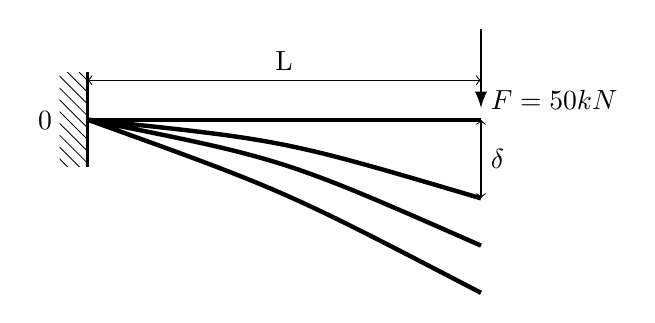
\begin{tikzpicture}
    %the points
    \point{origin}{-0.75}{-0.25};

    \point{begin}{0}{0};
    \point{end}{5}{0};
    \point{end_bot}{5}{-1};
    %the beam
    \beam{2}{begin}{end};
    %the support
    \support{3}{begin}[-90];
    %the load
    \load{1}{end}[90]   ;
    %the inscription of the load
    \notation{1}{origin}{0};
    \notation{1}{end}{$F=50kN$};

     \draw[<->] (end) -- (end_bot) node[midway, right] {$\delta$} ;
     \draw[<->] (0,0.5) -- (5,0.5) node[midway, above] {L};
     
    %the deflection curves
    \draw
      [-, ultra thick] (begin) .. controls (2.5, -.26) .. (5, -1)
      [-, ultra thick] (begin) .. controls (2.5, -.5) .. (5, -1.6)
      [-, ultra thick] (begin) .. controls (2.5, -.9)   .. (5, -2.2);
  \end{tikzpicture}
\label{fig:beam}   
}
%\raggedright
%\hfill
\subfloat[Possible cross-section shapes.]{
\centering

\begin{tikzpicture}
\vspace{1cm}

%%%%%
\tstar{0.25}{0.5}{6}{0}{thick,fill=yellow}
\tstar{0.14}{0.28}{6}{0}{thick,fill=white}

\tstar{0.25}{0.5}{6}{0}{thick,fill=yellow,xshift=-1.2cm}
\tstar{0.08}{0.16}{6}{0}{thick,fill=white,xshift=-1.2cm}

\tstar{0.25}{0.5}{6}{0}{thick,fill=yellow,xshift=-2.4cm}

%%%%%
\def\pos{1.2}
\fill[black] (\pos-0.24,-0.5) -- (\pos-0.24,0.5) -- (\pos+0.24,0.5)  -- (\pos+0.24,-0.5)   -- cycle ;
\fill[black] (\pos-0.5,-0.5) -- (\pos-0.5,-0.18) -- (\pos+0.5,-0.18)  -- (\pos+0.5,-0.5)   -- cycle ; 
\fill[black] (\pos-0.5,0.18) -- (\pos-0.5,0.5) -- (\pos+0.5,0.5)  -- (\pos+0.5,0.18)   -- cycle ;  

\def\pos{2.4}
\fill[black] (\pos-0.19,-0.5) -- (\pos-0.19,0.5) -- (\pos+0.19,0.5)  -- (\pos+0.19,-0.5)   -- cycle ;
\fill[black] (\pos-0.5,-0.5) -- (\pos-0.5,-0.25) -- (\pos+0.5,-0.25)  -- (\pos+0.5,-0.5)   -- cycle ; 
\fill[black] (\pos-0.5,0.25) -- (\pos-0.5,0.5) -- (\pos+0.5,0.5)  -- (\pos+0.5,0.25)   -- cycle ;  

\def\pos{3.6}
\fill[black] (\pos-0.14,-0.5) -- (\pos-0.14,0.5) -- (\pos+0.14,0.5)  -- (\pos+0.14,-0.5)   -- cycle ;
\fill[black] (\pos-0.5,-0.5) -- (\pos-0.5,-0.32) -- (\pos+0.5,-0.32)  -- (\pos+0.5,-0.5)   -- cycle ; 
\fill[black] (\pos-0.5,0.32) -- (\pos-0.5,0.5) -- (\pos+0.5,0.5)  -- (\pos+0.5,0.32)   -- cycle ;  

\vspace{1.2cm}

%%%%%
\fill[green,even odd rule] (0,-1.2) circle (0.5) (0,-1.2) circle (0.33);
\draw (0,-1.2) circle (0.5) ;
\draw (0,-1.2) circle (0.33) 
; 
\fill[green,even odd rule] (-1.2,-1.2) circle (0.5)(-1.2,-1.2) circle (0.17);
\draw (-1.2,-1.2) circle (0.5) ;
\draw (-1.2,-1.2) circle (0.17) 
; 
\fill[green,even odd rule] (-2.4,-1.2) circle (0.5) ;
\draw (-2.4,-1.2) circle (0.5) ;

%%%%%
\def\pos{1.2}
\fill[blue,even odd rule]  (\pos-0.5,-1.7) -- (\pos-0.5,-0.7) -- (\pos+0.5,-0.7) -- (\pos+0.5,-1.7) -- cycle ;

\def\pos{2.4}
\fill[blue,even odd rule]  (\pos-0.5,-1.7) -- (\pos-0.5,-0.7) -- (\pos+0.5,-0.7) -- (\pos+0.5,-1.7) -- cycle   (\pos-0.25,-1.45) -- (\pos-0.25,-0.95) -- (\pos+0.25,-0.95) -- (\pos+0.25,-1.45) -- cycle ;

\def\pos{3.6}
\fill[blue,even odd rule]  (\pos-0.5,-1.7) -- (\pos-0.5,-0.7) -- (\pos+0.5,-0.7) -- (\pos+0.5,-1.7) -- cycle   (\pos-0.35,-1.55) -- (\pos-0.35,-0.85) -- (\pos+0.35,-0.85) -- (\pos+0.35,-1.55) -- cycle ;

  \end{tikzpicture}


\label{fig:beam_shape}    
}
\caption{Cantilever beam problem.}
\end{figure}

Therefore, the problem to model has two continuous variables: the length $L \in [10,20]$ (in $m$) and the surface  $S \in [1,2]$ (in $m^2$) and one categorical variable $ \tilde{I}$ with 12 levels. The tip deflection, at the free end, $\delta$ is given by $$ \delta = f( \tilde{I}, L,S) = \frac{F}{3E} \frac{L^3}{S^2\tilde{I}} $$

% 98 points
% \begin{table}[H]
% \centering
%  \caption{Results of the cantilever beam models}
% \small

% \resizebox{0.6\columnwidth}{!}{%
% \small

% \begin{tabular}{cccc}
%   method & kernel & RMSE (cm) $\ $   &$\ $ time (s) \\
%   \hline 
%   $mat\_GOWER \ $ & square exponential & 1.386& 6.98     \\   
%   $mat\_CR$ & square exponential & 1.160& 90.98 \\
%   $mat\_EHH$ & square exponential &  &  \\
%   \hdashline 
%   $mat\_GOWER \ $ & absolute exponential &3.240 & 3.02 \\
%   $mat\_CR$ & absolute exponential & 1.980 & 193.60 \\
%   $mat\_EHH$ & absolute exponential &  & \\
% \hline
% \end{tabular}
% }
% \label{tab:resDragon}
% \end{table}
    
To compare our models, we draw a 98 point LHS as training set and the validation set is a grid of $12\times30\times30=10800$ points. For both squared exponential and absolute exponential kernels, the RMSE, likelihood and computational time for every model are shown in~\tabref{tab:resCantilever}. We recall that squared exponential and absolute exponential kernels differ only on the continuous variables and are the same for the categorical part.
As expected, the computational time and the likelihood increase when the model is more complex. The DoE seems of sufficient size for this problem as the computed RMSE of~\eqnref{eq:RMSE} (\textit{i.e.}, the total displacement error) decreases with the model complexity.

\begin{table}[H]
\centering
 \caption{Results of the cantilever beam models}
\small

\resizebox{0.9\columnwidth}{!}{%
\small

\begin{tabular}{ccccc}
  Categorical kernel & Continuous kernel & Displacement error (cm) & $ \ $ Likelihood  &$\ $ Time (s) \\
  \hline 
  GD & squared exponential &1.3858 & 111.13&  8.02 \\   
  CR & squared exponential & 1.1604 & 162.26 & 89.1 \\
  EHH & squared exponential &0.1247 &
256.90 & 2769.4 \\
  \hdashline 
  GD & absolute exponential & 3.2403 & 74.48   & 14.71  \\
  CR & absolute exponential & 3.0918 & 99.00 & 260.1 \\
  EHH & absolute exponential & 2.0951& 102.48 & 19784\\
\hline
\end{tabular}
}
\label{tab:resCantilever}
\end{table}

In~\figref{corr_Cantilever}, we have drawn the correlation matrix found between the cross-section shape (the resulting $R_1$ correlation matrix) for the three models. On the figure below, the higher the correlation, the thicker the ellipse. 


\begin{figure}[H]
\begin{center}
	\subfloat[With GD kernel.]{
      \centering 
\includegraphics[clip=true, height=4.6cm, width=5cm]{images/Corr_plot_shape23.JPG} \label{corr_canti_gower}
     }  
	\subfloat[ With CR kernel.]{
      \centering
\includegraphics[clip=true, height=4.6cm, width=5cm]{images/Corr_plot_shape22.JPG} \label{corr_canti_cr}
     }  
	\subfloat[ With EHH kernel. ]{
      \centering 
\includegraphics[clip=true, height=4.6cm, width=5cm]{images/Corr_plot_shape.JPG} \label{corr_canti_ehh}
     }  
\includegraphics[clip=true, height=5cm, width=0.5cm]{images/leg.jpg}
\centering     
\caption{Correlation matrix $R_1^{cat}$  using different choices for $\Theta_1$ for the categorical variable $\tilde{I}$ from the cantilever beam problem.}
\label{corr_Cantilever}
\end{center} 
\end{figure}
     
As expected, we have 3 groups of 4 shapes depending on their respective thickness (respectively, the levels \{1,4,7,10\} the levels \{2,5,8,11\} and the levels \{3,6,9,12\}). The more the thickness is similar, the higher the correlation: the thickness has more impact than the shape of the cross-section on the tip deflection. However, given the database, two points with similar $L$ and $S$ values will have similar output whatever the cross-section. The effect of the cross-section on the output is always the same (in the form of $\frac{1}{\tilde{I}}$) leading to an high correlation after maximizing the likelihood. In~\figref{corr_canti_ehh}, with the EHH kernel, we can distinguish the 3 groups of 4 shapes and, because the correlations are close to 1, the homoscedastic hyperphere model~\cite{Pelamatti} would lead to the same correlation matrix.  Also, with the CR kernel of~\figref{corr_canti_cr}, the medium thick group \{2,5,8,11\} being correlated with both the full and the hollow group, its correlation values are the higher whereas the correlation hyperparameters associated to the two other groups are smaller. 
%Hence, CR can retrieve the three groups structure but can not obtain the high in-group correlations as the coefficients associated to both hollow and full group have to be smaller than the ones of the medium group. 
For the GD model in~\figref{corr_canti_gower}, there is only one mean positive correlation value as before.

\subsubsection{Aircraft design application ($n=10$, $ m=0$, $l=2$ and $L_1=9$, $L_2=2$) }
\label{subsec:aircraft}

The ``\texttt{DRAGON}'' aircraft concept %in~\figref{Dragon2020}
has been introduced by ONERA in 2019~\cite{schmollgruber} within the scope of the European CleanSky 2 program~\footnote{\href{https://www.cleansky.eu/technology-evaluator}{\color{blue}https://www.cleansky.eu/technology-evaluator}} which sets the objective of 30\% reduction of CO2 emissions by 2035 with respect to 2014 state of the art.
% \begin{figure}[H]
% \begin{center}
%   \begin{subfigure}[b]{.5\linewidth}
%       \centering
% 	\includegraphics[clip=true,height=4cm]{images/Dragon2020.pdf}
%       \end{subfigure}
% \end{center}    
%   \begin{subfigure}[b]{.48\linewidth}
%       \centering
% 	\includegraphics[height=5cm]{images/onera-dragon-21321165_wagner.jpg}
%       \end{subfigure}~~~
%       %
%       \begin{subfigure}[b]{.48\linewidth}
%       \centering 
% 	\includegraphics[clip=true,height=5cm]{images/0246270f-salon-du-bourget-2019-a-quoi-ressemblera-l-avion-du-futur__1200_900__0-418-3891-2612.jpeg}
%   \end{subfigure}
%   \caption{``\texttt{DRAGON}'' aircraft mock-up.}
%         \label{Dragon2020}
% \end{figure}    
The employment of a distributed propulsion comes at a certain cost; a turboelectric propulsive chain is necessary to power the electric fans which brings additional complexity and weight.
%as in~\figref{DragonArchitecture}. 
The turboelectric propulsive chain being an important weight penalty, it is of particular interest to optimize the chain and particularly the number and type of each component, characterized by some discrete values.  The definition of the architecture variable is given in~\tabref{tab:dragon_archi1} and the definition of the turboshaft layout is given in~\tabref{tab:dragon_archi2}. For the sake of simplicity, we restrict the optimization problem to the case of two electric cores and generators but more optimizations have been performed in~\cite{SciTech_cat}.

%
%\begin{figure}[H]
%\vspace*{-0.6cm}
%
%  \centering 
%\includegraphics[clip=true,,height=6cm]{images/DragonArchitecture.pdf}
% \caption{Turboelectric propulsive architecture.}
% \label{DragonArchitecture}
%\label{Dragon}
%\end{figure} 

\begin{table}[H]
\centering
\vspace*{-0.1cm}

 \subfloat[Definition of the architecture variable and its 9 associated levels.]{
\small

\resizebox{0.8\columnwidth}{!}{%
\small

\begin{tabular}{cccc}
  Architecture number $\ $ & Number of motors $\ $ & Number of cores $\ $ & Number of generators $\ $ \\
  \hline
  1 & 8 &2 & 2\\
  2 & 12 & 2 & 2\\
  3 & 16 & 2 & 2\\
  4 &20 &2 & 2\\
  5 & 24 & 2 & 2\\
  6 & 28 & 2 & 2\\
  7 &32 & 2 & 2\\
  8 & 36  & 2 & 2\\
  9 & 40 & 2 & 2\\

\hline
\end{tabular}
}
\label{tab:dragon_archi1}
}
\centering
\vspace*{+0.1cm}

\subfloat[Definition of the turboshaft layout variable and its 2 associated levels.]{
\small

\resizebox{0.8\columnwidth}{!}{%
\small

\begin{tabular}{cccccc}
  Layout & Position & y ratio & Tail & VT aspect ratio & VT taper ratio\\
  \hline 
  1 & under wing &0.25 & without T-tail& 1.8 & 0.3 \\
  2 & behind & 0.34 & with T-tail& 1.2 & 0.85\\
 
\hline
\end{tabular}
}
\label{tab:dragon_archi2}
}
\caption{Categorical variable definition}
\end{table}
The analysis of ``\texttt{DRAGON}'' is treated with Overall Aircraft Design method in FAST-OAD~\cite{David_2021}.  We are considering the following problem described in~\tabref{tab:dragon}.
\begin{table}[H]
\centering
\vspace*{-0.3cm}

 \caption{Definition of the ``\texttt{DRAGON}'' optimization problem.}
\small

\resizebox{1.0\columnwidth}{!}{%
\small

\begin{tabular}{lllrr}
 & Function/variable & Nature & Quantity & Range\\
\hline
\hline
Model & Fuel mass & cont & 1 &\\
\hline
with respect to & \mbox{Fan operating pressure ratio} & cont & 1 & $\left[1.05, 1.3\right]$ \\  
     & \mbox{Wing aspect ratio} & cont & 1 &    $\left[8, 12\right]$ \\
    & \mbox{Angle for swept wing} & cont & 1 & $\left[15, 40\right]$  ($^\circ$) \\
     & \mbox{Wing taper ratio} & cont & 1 &    $\left[0.2, 0.5\right]$ \\
     & \mbox{HT aspect ratio} & cont & 1 &    $\left[3, 6\right]$ \\
    & \mbox{Angle for swept HT} & cont & 1 & $\left[20, 40\right]$  ($^\circ$) \\
     & \mbox{HT taper ratio} & cont & 1 &    $\left[0.3, 0.5\right]$ \\
 & \mbox{TOFL for sizing}  & cont &1 & $\left[1800., 2500.\right]$ ($m$) \\
 & \mbox{Top of climb vertical speed for sizing $ \ $} & cont & 1 & $\left[300., 800.\right]$($ft/min$) \\
 & \mbox{Start of climb slope angle} & cont & 1 & $\left[0.075., 0.15.\right]$($rad$) \\

 & \multicolumn{2}{l}{Total  continuous variables} & 10 & \\
 \cline{2-5}
& \mbox{Architecture} & cat & 9 levels & \{1,2,3, \ldots,7,8,9\} \\
& \mbox{Turboshaft layout} & cat & 2 levels & \{1,2\} \\

 & \multicolumn{2}{l}{Total categorical variables} & 2 & \\
 \cline{2-5}

  &   \multicolumn{2}{l}{\textbf{Total relaxed variables}} & {\textbf{21}} & \\
  \hline

\end{tabular}
}
\label{tab:dragon}
\end{table}

Twice, we draw  $250$ points by LHS. Over the first DoE, that is the training set, we build the model to predict the fuel mass and over the second one, we validate our prediction and compute the RMSE reported in~\tabref{tab:resDragon}.
In this case, the number of hyperparameters is 12 for GD kernel, 21 for CR kernel and 47 for EHH kernel. Evaluating the function is costly, around 4 minutes for a single point. We observed similar performances for all models, the performance is mostly determined by the choice of the continuous kernel. 
For a problem that has that many variables, it seems useless and impractical to use a complicated model, the GD kernel being already performing well. 
On~\figref{corr_turboelectric}, we plot, for the three kernels, the approximate correlation matrices for the first categorical variable. As we can see, when considering the general EHH kernel, as in~\figref{corr_turboelectric_ehh}, the closer the levels, the higher the correlation. In fact, in this case, the only difference between two levels is the number of motors. Therefore, the more similar the number of motors, the more similar the fuel consumption. Given that, we expect, when considering CR kernel as in~\figref{corr_turboelectric_cr} that the higher correlation should appear "in the middle" \{4,5,6\} as these levels are meant to be the most correlated with the others. This is what happens to a certain extent but the levels 7 and 8 are weirdly appearing too much correlated with one another. This could be a numerical problem, the optimization being hard with that many variables and hyperparameters. As before, the GD kernel is the less precise and just give a mean correlation over the whole space as in~\figref{corr_turboelectric_gower}. In~\figref{corr_turboshaft}, we plot, for the three methods, the approximated correlation matrices for the second categorical variable. There is only two engine layouts so there is only one correlation. In this case, the correlation is positive indicating that the plane behave in the same way no matter the layout.


\begin{table}[H]    
\centering
 \caption{Results of the aircraft models based on a 250 point validation set}
\small
\resizebox{0.8\columnwidth}{!}{%
\small

\begin{tabular}{ccccc}
  kernel& $ \ $ number of hyperparameters  & $\ $  kernel   & $\ $fuel error (kg) $\ $  & time (s)   \\
  \hline 
  GD & 12 & squared exponential & 2115 & 65 \\
  CR & 21 & squared exponential & 2068  & 210  \\
  EHH & 47 & squared exponential & 2147 &  9450\\
   \hdashline 
  GD & 12 & absolute exponential &1666 & 65 \\
  CR & 21 & absolute exponential & 1664  & 210 \\
  EHH & 47 & absolute exponential & 1593 &  9295 \\
\hline
\end{tabular}
}
\label{tab:resDragon}
\end{table}



\begin{figure}[H]
\begin{center}
	\subfloat[GD kernel.]{
      \centering 
\includegraphics[clip=true, height=4.4cm, width=5cm]{images/Corr_9_archi_gower.JPG} \label{corr_turboelectric_gower}
     }  
	\subfloat[CR kernel.]{
      \centering 
\includegraphics[clip=true, height=4.4cm, width=5cm]{images/Corr_9_archi_cr.JPG} \label{corr_turboelectric_cr}
     }  
	\subfloat[EHH kernel.]{
      \centering 
\includegraphics[clip=true,  height=4.4cm, width=5cm]{images/Corr_9_archi.JPG}
\label{corr_turboelectric_ehh}
     }  
\includegraphics[clip=true, height=4.7cm, width=0.5cm]{images/leg.jpg}
\centering     
\caption{Correlation matrix $R_1^{cat}$  using different choices for $\Theta_1$  for the turboelectric architecture variable.}
\label{corr_turboelectric}
\end{center} 
\end{figure}



\begin{figure}[H]
\begin{center}
\vspace{-1cm}
	\subfloat[GD kernel.]{
      \centering 
\includegraphics[clip=true, height=4.4cm, width=5cm]{images/Corr_9_archi2_gower.JPG} \label{corr_turboshaft_gower}
     }  
	\subfloat[CR kernel.]{
      \centering 
\includegraphics[clip=true, height=4.4cm, width=5cm]{images/Corr_9_archi2_cr.JPG} \label{corr_turboshaft_cr}
     }  
	\subfloat[EHH kernel.]{
      \centering 
\includegraphics[clip=true, height=4.4cm, width=5cm]{images/Corr_9_archi_2.JPG} \label{corr_turboshaft_ehh}
     }  
\centering
\includegraphics[clip=true, height=4.65cm, width=0.5cm]{images/leg.jpg}
\caption{Correlation matrix $R_2^{cat}$  using different choices for $\Theta_2$  for the turboshaft layout variable.}
\label{corr_turboshaft}
\end{center} 
\end{figure}

One can note that increasing the number of motors or changing a layout will not change the way an aircraft flies. For example, having more motors will only increase the fuel consumption by a given factor. The latter will always remain positive and related to the continuous variables. Hence, in this test case, we do not have opposite effects between two categorical levels.

In most industrial applications, radically opposite effects over a complex system do not occur so often. For instance, on the industrial applications that can be found on the literature, there was not a clear need for negative correlation values~\cite{Pelamatti,Roustant, cuesta2021comparison}. Therefore, in practice, the exponential model is not that limiting compared to the homoscedastic hypersphere model.  





% \subsubsection{Categorical Branin function}

% Let the function $f$ to model be the modified categorical Branin function~\cite{Gower}. This problem has 3 variables: two continuous variables in $[0,1]$ and one categorical variable with three levels and the two first levels are totally correlated. 
% We draw a DoE of $60$ points by LHS to compare the given GP models and compute the error terms.
% To begin with, we start by plotting the models built with the different methods in~\figref{models_hal5} and compute their respective RMSE to compare them with the original formulation of the methods.
% The obtained values are given in~\figref{models_hal5} from a validation base of size 30603 that corresponds to 101 points from 0 to 1 in every continuous direction for every level (see Appendix~\ref{subsec:branin} for a detailed description of the function).

% \begin{figure}[H]
% \begin{center}
%   \subfloat[Our model (with $\Theta_1=mat\_CR$): RMSE = 60.707]{
%       \centering
% 	\includegraphics[clip=true, height=4cm, width=12cm]{images/CP_CR_Hal5.png}} 

% 	\subfloat[Our model (with $\Theta_1=mat\_GOWER$): RMSE = 77.793]{
%       \centering 
% 		\includegraphics[clip=true, height=4cm, width=12cm]{images/CP_GOWER_Hal5.png}
%      }  
     
%     % (Homoscedastic hypersphere, RMSE= 63.021
%     \subfloat[Our model (with $\Theta_1=mat\_EHH$): RMSE = 60.721 ]{
%       \centering 
% 	\includegraphics[clip=true, height=4cm, width=12cm]{images/CP_HOMO_Hal5.png}}

% 	    \subfloat[Our model (with $\Theta_1=mat\_FULL$): RMSE = 60.707  ]{
%       \centering 
% 		\includegraphics[clip=true, height=4cm, width=12cm]{images//CP_FULL_Hal5.png}
%     }

% \caption{Mean predictions (over the three levels) for the categorical Branin problem using a DoE of 60 points (in red in the curve plots). }\label{models_hal5}
% \end{center} 
% \end{figure}


% In this test case, we clearly show that the full model, the continuous relaxation model and the square exponential homoscedastic one are the same. However, we still have numerical instabilities but using the square exponential homoscedastic kernel as proposed in this paper instead of using the raw matrix leads to a better estimation of the hyperparameters. For homoscedastic hypersphere, the RMSE that we found is 63.021. The Gower distance model is the only one that differs visually and that differs consequently in error from the others (77.8 instead of 60.7). As mentioned in Section~\ref{subsec:hyp_res}, with 3 levels, square exponential homoscedastic hypersphere and continuous relaxation are equivalent methods, so these results were theoretically expected. However, when comparing with the original homoscedastic hypersphere, the square exponential model differs as the third level is negatively correlated from the two others and because the square exponential kernel returns only positive value. In this case, the estimated correlation is 0.03 with the square exponential kernel against -0.15 with the original one. 


%% !TeX spellcheck = en_GB
%!TEX root = ../side-constrained.tex

\section{Conclusion}

We provided a counterexample to a claimed existence result for dynamic equilibria with side constraints. The implications of this counterexample were shown to be severe since solutions to the canonical infinite dimensional variational inequality are in some sense useless and other approaches seem to be necessary. 
We then established a general framework for defining side-constrained dynamic equilibria based on two key objects: A \setS{} $S$ containing all feasible flows (given as walk inflows) and correspondences $A_p$ providing the flow-dependent set of \addmEpsDev s. We showed that this equilibrium concept not only encompasses the known unconstrained equilibria with and without departure time choice and capacitated dynamic equilibria with convex \setS{}s but also allows for a whole range of new dynamic equilibria inspired by static side-constrained equilibria.
We provided conditions under which they can be characterized as solutions to a quasi-variational or even a variational inequality. The latter characterization then also gave rise to a first existence result for certain side-constrained dynamic equilibria with convex \setS.
Finally, we turned to equilibria wherein the side-constraints are given by time-varying edge-load constraints. To deal with the non-convexity of the \setS{}, we employed an augmented Lagrangian approach by relaxing the hard edge-load-capacities and replacing them by penalty functions. We demonstrated that these existence results apply, in particular, for the widely used Vickrey point queue model as well as the linear edge delay model.

Several important questions remain open. First of all, it would be interesting to find an existence result for BSDE similar to \Cref{thm:ExistenceFDAddSpaceExCP} for LPDE and MNSDE. The main obstacle to obtaining such a result seems to be the fact that for BSDE, the definition of \addmEpsDev s involves the network loading which, in general, is a very complex mapping and, even for well-studied flow models, is not fully understood yet. Note that, due to \Cref{prop:RelationshipsOfCDE}, such a result would also directly imply existence of \globalEL{} as well as providing an alternative proof for the existence of LPDE. Another aspect is the multiplicity of equilibria and
the issue of selecting a particular type of equilibrium having desirable properties.
It is an interesting research direction to characterize equilibrium concepts
that admit equilibrium selection via appropriate optimization or optimal control reformulations
whose optimal solutions provide such desirable properties.
\section{Conclusion}
\label{sec:conclu}

In this work, we have proposed a class of kernels for GP models that extends the exponential continuous kernels to the mixed-categorical setting. We showed that this class of kernels generalizes Gower distance and continuous relaxation based kernels. A classification between the proposed kernels as well as a proof of the SPD nature of the resulting correlation matrices have been also proposed. Numerical illustrations on analytical toy problems showed the good potential of the proposed kernels to reduce the number of hyper-parameters and thus the computational time. The implementation of our proposed method has been released in the toolbox SMT v1.4\footnote{\url{https://smt.readthedocs.io/en/latest/}}. 
%These GP models are often used for BO, and, as we generalized the continuous relaxation kernel, the previous works that optimized a deep learning model can naturally be extended by our method.  


When considering complex kernels, a good approach would be to use a model reduction technique such as Kriging with Partial Least Squares (KPLS)~\cite{Bouhlel18} that is derived from the construction of the correlation matrix via a kernel function. KPLS is an adaptation of the Partial Least Squares regression for exponential kernels and is used to reduce the number of hyperparameters and handle a large number of mixed inputs. Further works will consider to include such dimension reduction techniques to improve the computational efficiency of our model  and tackle higher dimensional problems. 




\section*{Acknowledgements}
This work is part of the activities of ONERA - ISAE - ENAC joint research group. The research presented in this paper has been performed in the framework of the AGILE 4.0 project (Towards Cyber-physical Collaborative Aircraft Development) and has received funding from the European Union Horizon 2020 Programme under grant agreement n${^\circ}$ 815122. 
We thank Raul Carreira Rufato (ISAE-Supaero MSc) for his contribution to Gower distance implementation, and Dr. Eric Nguyen Van (ONERA) and Christophe David (ONERA) for their contribution to DRAGON aircraft design.
The authors are grateful to the partners of the AGILE 4.0 consortium for their contribution and feedback.
%\newpage


%We briefly explain the algebraic background relevant for the definition of the the main character of this paper: the element $A \in \HF(\tau^{-1})$.
We follow the conventions for $A_{\infty}$-machinery from \cite{seidelbook}.

Suppose $\mathcal{A}$ is a homologically unital $A_\infty$-category. The Yoneda embedding is a functor
\[
\mathcal{Y} \colon \mathcal{A} \rightarrow mod_{\mathcal{A}}
\]
taking an object $L$ to the $\mathcal{A}$-module 
$\mathcal{Y}(L)$
defined by
\[
\mathcal{Y}(L)(K) := Mor_{\mathcal{A}}(K,L).
\]
and 
\[
\mu^d_{\mathcal{Y}(L)}(b,a_{d-1}, \dots, a_1) := \mu^d(b, a_{d-1}, \dots , a_1)
\]
for $a_i \in Mor_{\mathcal{A}}(K_{i-1},K_i)$, $i\in \{1, \dots , d-1\}$ 
and $b \in \mathcal{Y}(L)(K_{d-1}) = Mor_{\mathcal{A}}(K_{d-1},L)$.

By \cite[Section 2g]{seidelbook} the Yoneda embedding induces a unital, full and faithfull embedding
\[
\Homol(\mathcal{Y}) \colon \Homol(\mathcal{A}) \to \Homol(mod_{\mathcal{A}}).
\]
The derived cateogory $\mathcal{DA}$ of $\mathcal{A}$
can be constructed as follows: Take a triangulated completion of the image of $\mathcal{Y}$ in $mod_{\mathcal{A}}$ and take its homology category.

The following is an immediate consequence of the properties of the Yoneda embedding. 

\begin{cor}
 Each $f\in Mor_{D\mathcal{A}}(\mathcal{Y}(L_1), \mathcal{Y}(L_2))$ can be represented by 
 $\mathcal{Y}(\alpha)$
 for some $\alpha \in Mor_{\mathcal{A}}(L_1,L_2)$. 
 Moreover, $[\alpha]\in Mor_{H(\mathcal{A})}(L_1,L_2)$ is uniquely defined. 
 \end{cor}
 \begin{proof}
First, note that
\[
Mor_{D\mathcal{A}}(\mathcal{Y}(L_1), \mathcal{Y}(L_2))
\cong \Homol(Mor_{mod_{\mathcal{A}}}(\mathcal{Y}(L_1), \mathcal{Y}(L_2))).
\]
 For any object $K$, $\mathcal{Y}(\alpha)$ determines the map
 \[
 \mathcal{Y}(L_1)(K) \cong Mor(K,L_1) \xrightarrow{\mu^2(\alpha,-)}  
 Mor(K,L_2) \cong \mathcal{Y}(L_2)
 \]
 The existence and uniqueness of $\alpha$ follow immediately from $\Homol(\mathcal{Y})$ being full and faithful.
\end{proof}

\noindent
These notions are applied in this paper to the $A_{\infty}$-category $\mathcal{F}uk(M)$.
 



%%%%%%%%%%%%%%%%%%%%%%%%%%%%%%%%%%%%%%%%%%%%%%%%%%%%%%%%%%%%%%%%%%%%%%%%%%%%
%%%%%%%%%%%Homological Version%%%%%%%%%%%%%%%%%%%%%%%%%%%%%%%%%%%%%%%%%%%%%%
%%%%%%%%%%%%%%%%%%%%%%%%%%%%%%%%%%%%%%%%%%%%%%%%%%%%%%%%%%%%%%%%%%%%%%%%%%%%
\begin{comment}
\subsection{$A_\infty$-categories}
We work in a homological setting, in contrast to Seidel's book.
Moreover, we work in an ungraded setting, maybe later updated to a $\Z / 2\Z$-grading.

We briefly recall here the main definitions and fix notation.

Suppose $\mathcal{A}$ is a homologically unital $A_\infty$-category. The Yoneda embedding is a functor
\[
\mathcal{Y} \colon \mathcal{A} \rightarrow mod_{\mathcal{A}}
\]
taking an object $L$ to the $\mathcal{A}$-module 
$\mathcal{Y}(L)$
defined by
\[
\mathcal{Y}(L)(K) := Mor_{\mathcal{A}}(K,L).
\]
and 
\[
\mu^{\mathcal{Y}(L)}(a_1, \dots, a_{n-1},b) := \mu_n(a_1, \dots , a_{n-1},b)
\]
for $a_i \in Mor_{\mathcal{A}}(K_i,K_{i+1})$, $i\in \{1, \dots , n-1\}$ 
and $b \in \mathcal{Y}(L)(K_n) = Mor_{\mathcal{A}}(K_n,L)$.

By Seidel, section 2g, the Yoneda embedding induces a unital, full and faithfull embedding
\[
H(\mathcal{Y}) \colon H(\mathcal{A}) \to H(mod_{\mathcal{A}}).
\]

The derived cateogory $\mathcal{DA}$ of $\mathcal{A}$
can be constructed as follows: Take a triangulated completion of $mod_{\mathcal{A}}$ and take its homology category.

The following is an immediate consequence of the properties of the Yoneda embedding. We include it here, since it is relevant for this article.

\begin{cor}
 Each $f\in Mor_{D\mathcal{A}}(\mathcal{Y}(L_2), \mathcal{Y}(L_1))$ can be represented by 
 $\mathcal{Y}(\alpha)$
 for some $\alpha \in Mor_{\mathcal{A}}(L_2,L_1)$. 
 Moreover, $[\alpha]\in Mor_{H(\mathcal{A})}(L_2,L_1)$ is uniquely defined. 
 For any object $K$, $\mathcal{Y}(\alpha)$ determines the map
 \[
 \mathcal{Y}(L_2)(K) \cong Mor(K,L_2) \xrightarrow{\mu_2(-,\alpha)}  
 Mor(K,L_1) \cong \mathcal{Y}(L_1)
 \]
 
\end{cor}
\begin{proof}
First, note that
\[
Mor_{D\mathcal{A}}(\mathcal{Y}(L_2), \mathcal{Y}(L_1))
\cong H(Mor_{mod_{\mathcal{A}}}(\mathcal{Y}(L_2), \mathcal{Y}(L_1))).
\]


First, note that
\[
Mor_{D\mathcal{A}}(\mathcal{Y}(L_2), \mathcal{Y}(L_1))
\cong H(Mor_{mod_{\mathcal{A}}}(\mathcal{Y}(L_2), \mathcal{Y}(L_1))) \cong Mor_{H({\mathcal{A}})}(\mathcal{Y}_H(L_2), \mathcal{Y}_H(L_1)),
\]
where $\mathcal{Y}_H(L) = H(Mor_\mathcal{A}(K,L))$.
So $f$ consists of a collection of maps $f(K) \colon Mor_{H(\mathcal{A})}(K,L_2) \to Mor_{H(\mathcal{A})}(K,L_1)$
for every object $K$.

The existence and uniqueness of $\alpha$ follow immediately from $H(\mathcal{Y})$ being full and faithful.
\end{proof}

\end{comment}


%\newpage
\section{Appendix}

To begin with, in Appendix~\ref{apendix:EHH2CR},  we give the parameterization that allows us to obtain the continuous relaxation model from our more general one. 
Then, this appendix describes the two analytical test cases more in details. In Appendix~\ref{subsec:red_blue}, a description of the blue/red case is given and in Appendix~\ref{subsec:cosine}, the cosine test case is detailed. 

\subsection{Continuous relaxation is a particular instance of our proposed FE Kernel.} \label{apendix:EHH2CR}
To show that CR is a particular instance of FE, it suffices to show that the matrix $\Phi(\Theta_i)$ is diagonal whenever $\Theta_i$ is set to a diagonal one. In fact, assume that we have, in our general model, $[\Theta_i]_{j \neq j'} = 0, \  \forall (j,j') \in \{ 1, \ldots, L_i \}.$ 
Knowing that $\cos(0)=1$ and $\sin(0)=0$, the matrix $C(\Theta_i)$ writes as  \\
$$C(\Theta_i) = \begin{bmatrix}
1 & 0 & 0  & 0  \\
1  & 0 &  \ldots & 0 \\
\vdots &\vdots & \ddots & 0 \\
1 &  0 & 0  & 0 \\
\end{bmatrix} \quad \mbox{ and } \quad  C(\Theta_i) C(\Theta_i)^\top = \begin{bmatrix}
1 & 1 & 1  & 1  \\
1  & 1 &  \ldots & 1 \\
\vdots &\vdots & \ddots & 1 \\
1 &  1 & 1  & 1 \\
\end{bmatrix} $$
Therefore, we also have 
$$[\Phi(\Theta_i)]_{j \neq j'} = \frac{\log \epsilon }{2} ([C(\Theta_i) C(\Theta_i)^\top]_{j,j'} -1) = 0 \  \forall (j,j') \in \{ 1, \ldots, L_i \} $$ that is the continuous relaxation kernel. \qed \mbox{}\\ 

\subsection{2D blue/red test case}
\label{subsec:red_blue}
This test case has one categorical variable with two levels: 'blue' or 'red' and one continuous variable in $[0,4]$.
\begin{itemize}
    \item The blue DoE of 3 points is the following: x= $\{0,1,4\}$, y=$\{0,9,16\}$
    \item The red DoE of 4 points is the following: x= $\{0,1,2,3\}$, y=$\{0,1,8,27\}$
\end{itemize}
Therefore, we have a DoE consisting of 7 points either blue or red, with continuous value ranging between 0 and 4 and taking value between 0 and 27.



\subsection{Categorical cosine case}
\label{subsec:cosine}
This test case has one categorical variable with 13 levels and one continuous variable in $[0,1]$~\cite{Roustant}.
Let $w= (x,c )$ be a given point with  $x$ being the continuous variable and $c$ being the categorical variable, $c \in \{1, \ldots, 13\}$.

\begin{equation*}
\begin{split}
f(w) &= \cos \left( \frac{7 \pi}{2} x + \left( 0.4 \pi  + \frac{\pi }{15} c  \right) - \frac{c}{20} \right) , ~~~\mbox{if c $\in\{10,\ldots,9\}$ }  \\
f(w) &= \cos \left( \frac{7 \pi}{2} x  - \frac{c}{20} \right) , ~~~\mbox{if c $\in\{10,\ldots,13\}$ }  \\
\end{split}
\end{equation*}
The reference landscapes of the objective function (with respect to the categorical choices) are drawn on~\figref{fig:Roustant_ref}.

\begin{figure}[H]
\centering
\includegraphics[scale=.15]{images/Roustant_curves.png}
\caption{Landscape of the cosine test case from~\cite{Roustant}.}
\label{fig:Roustant_ref}    
\end{figure}
The DoE is given by a LHS of 98 points.
% Our DoE drawn by LHS is the following: 
% $x= \left\{ \vphantom{[]^2}\right.$[ 0.65605253,  6.        ],
%       [ 0.83350264,  4.        ],
%       [ 0.15026485,  7.        ],
%       [ 0.24143059, 12.        ],
%       [ 0.03096315,  8.        ],
%       [ 0.23260394,  9.        ],
%       [ 0.21316332, 11.        ],
%       [ 0.80211976,  4.        ],
%       [ 0.94950991,  1.        ],
%       [ 0.58874134,  2.        ],
%       [ 0.15866055,  8.        ],
%       [ 0.29988981,  4.        ],
%       [ 0.11186171,  4.        ],
%       [ 0.3476918 ,  2.        ],
%       [ 0.01205944,  3.        ],
%       [ 0.71141884,  8.        ],
%       [ 0.28951039,  5.        ],
%       [ 0.73724151,  9.        ],
%       [ 0.38762527,  0.        ],
%       [ 0.3443474 ,  1.        ],
%       [ 0.31419979,  0.        ],
%       [ 0.97505473,  0.        ],
%       [ 0.71769637, 11.        ],
%       [ 0.14208871,  9.        ],
%       [ 0.02645321, 11.        ],
%       [ 0.64144679,  4.        ],
%       [ 0.93347456,  1.        ],
%       [ 0.26023608,  4.        ],
%       [ 0.36179242, 11.        ],
%       [ 0.19235854,  3.        ],
%       [ 0.82539539, 12.        ],
%       [ 0.77423165,  1.        ],
%       [ 0.62454224,  5.        ],
%       [ 0.56235338,  4.        ],
%       [ 0.68487501, 12.        ],
%       [ 0.52396804,  6.        ],
%       [ 0.31718476,  9.        ],
%       [ 0.49061463,  6.        ],
%       [ 0.69566705,  2.        ],
%       [ 0.60557496,  2.        ],
%       [ 0.90013372,  2.        ],
%       [ 0.77980976,  2.        ],
%       [ 0.99262069,  6.        ],
%       [ 0.61237851,  9.        ],
%       [ 0.07168795,  2.        ],
%       [ 0.37433399,  3.        ],
%       [ 0.51563867,  7.        ],
%       [ 0.06439778,  6.        ],
%       [ 0.39792487, 10.        ],
%       [ 0.09111936,  2.        ],
%       [ 0.54844499, 10.        ],
%       [ 0.6778083 ,  0.        ],
%       [ 0.10018382,  3.        ],
%       [ 0.78794137,  0.        ],
%       [ 0.48618283,  0.        ],
%       [ 0.64305827,  7.        ],
%       [ 0.98717047,  4.        ],
%       [ 0.92111218, 11.        ],
%       [ 0.9095025 ,  5.        ],
%       [ 0.42987802, 10.        ],
%       [ 0.5931088 ,  6.        ],
%       [ 0.57328161,  7.        ],
%       [ 0.85035836, 11.        ],
%       [ 0.04171931,  5.        ],
%       [ 0.96455513, 11.        ],
%       [ 0.05890046,  2.        ],
%       [ 0.28382111,  2.        ],
%       [ 0.81016573,  5.        ],
%       [ 0.00382184,  7.        ],
%       [ 0.8454141 ,  8.        ],
%       [ 0.93911432,  8.        ],
%       [ 0.66928872, 11.        ],
%       [ 0.12230256, 11.        ],
%       [ 0.20098996,  6.        ],
%       [ 0.25362715,  7.        ],
%       [ 0.75857015,  4.        ],
%       [ 0.18005584,  8.        ],
%       [ 0.55734768, 11.        ],
%       [ 0.44058174,  7.        ],
%       [ 0.21558225,  3.        ],
%       [ 0.88253717,  3.        ],
%       [ 0.42716698, 12.        ],
%       [ 0.7281732 ,  0.        ],
%       [ 0.27491291,  7.        ],
%       [ 0.16597145,  8.        ],
%       [ 0.86510046,  2.        ],
%       [ 0.46646275, 12.        ],
%       [ 0.39911793,  9.        ],
%       [ 0.12286505,  1.        ],
%       [ 0.33037   ,  1.        ],
%       [ 0.86803419,  6.        ],
%       [ 0.47060982, 12.        ],
%       [ 0.44960284,  4.        ],
%       [ 0.89443379,  3.        ],
%       [ 0.53266967,  5.        ],
%       [ 0.41534775,  6.        ],
%       [ 0.50583278,  0.        ],
%       [ 0.75433057, 10.        ]$\left.\vphantom{[]^2}\right\}$
Our validation set is a evenly spaced grid of 1000 points in $x$ ranging  for every of the 13 categorical levels  for a total of 13000 points.



%\nocite{*}
%\bibliography{sample}
\bibliography{sample}
%%%%%%%%%%%%%%%%%%%%%%%%%%%%%%%%%%%%%%%%%%%%%%%%%%%%%%%%%%%%%%%%%%%%%%
\end{document}